\documentclass[msc, classic, a4paper]{ufbathesis}
\usepackage[utf8]{inputenc}
\usepackage[brazil]{babel}
\usepackage{fancyvrb}
\usepackage[alf]{abntex2cite}
\usepackage{graphicx}
\usepackage{multicol}
\usepackage{enumitem}
\usepackage{float}
\usepackage{rotating}
\usepackage{tipa}
\usepackage{textcomp}
\usepackage{multirow}
\DeclareGraphicsExtensions{.pdf}

\defenseyear{2016}
\date{08 de Julho de 2016}
\adviser[f]{Profa. Dra. Christina von Flach G. Chavez}
\coadviser{Prof. Dr. Paulo Roberto Miranda Meirelles}

\title{
  Um estudo sobre a complexidade estrutural e o custo de mudança das
  ferramentas de análise estática de código-fonte
}

\author{Joenio Marques da Costa\\
  {\small joenio@joenio.me}
}

\begin{document}

\frontpage
\frontmatter
\presentationpage

\resumo

(pendente)

\begin{keywords}

  (pendente)

\end{keywords}

\tableofcontents
\listoffigures
\listoftables

\mainmatter

%------------------------------------------%

\xchapter{Introdução}{}

%Modularity
%Modularity describes the logical partitioning of software into several parts, components, and modules.
%Software will be easy to understand and change when composed of independent modules.
%Simplicity
%Software simplicity to the extent that it lacks complexity in organization, language, and
%implementation techniques and reflects the use of singularity concepts and basic structures.
%sao dois faotes citados em TABLE-II: FACTORS REPORTED IN [21]
%21 = David E. Peercy, “A Software Maintainability Evaluation
%Methodology”, IEEE Transactions on Software Engineering,
%Vol. SE-7, NO. 4, July 1981.
%
%Complexity
%The complexity of a software affects its maintainability. It is supposed to reflect to a certain extent, the
%difficulty in comprehending or maintaining codes. é um dos fatores que afetam a manutenabilidade
%TABLE-III: FACTORS REPORTED IN [17]
%17 = Khairuddin Hashim and Elizabeth Key,” A Software
%Maintainability Attributes Model”, Malaysian Journal of
%Computer Science, Vol. 9 No. 2, December 1996, pp. 92-97
%
%Average
%Cyclomatic
%Complexity
%Average Cyclomatic Complexity can be expressed as the average of cyclomatic complexities of all
%modules.
%TABLE-IV: FACTORS REPORTED IN [18]
%18 = K.K. Aggarwal, Yogesh Singh, Pravin Chandra and
%Manimala Puri,” Measurement of Software Maintainability
%Using a Fuzzy Model”, Journal of Computer Sciences 1 (4):
%538-542, 2005 ISSN 1549-3636 © 2005 Science
%Publications
%
%
%Simplicity
%Software size and its complexity is a very critical issue. The code smell “DuplicateCode” is, perhaps,
%the worst [7]. It takes longer to identify a specific class when there are many classes. The presence of
%several classes that are almost empty is a sign of code that may possess low maintainability.
%TABLE-V: FACTORS REPORTED IN [12]
%12 = B. Anda, “Assessing Software System Maintainability using
%Structural Measures and Expert Assessments,” in IEEE
%International Conference Software Maintenance, 2007, pp.
%204–213.
%
%\cite{A Survey of Key Factors Affecting Software Maintainability}
%
%
%We will also
%investigate the maintainability measures taxonomy by
%Oman et al where 92 measures are listed and classified [24].
%[24] Oman, P., Hagemeister, J., and Ash, D., A Definition
%and Taxonomy for Software Maintainability, report
%SETL Report 91-08-TR, University of Idaho, 1991.
%
%\cite{Measurements of Software Maintainability}
%
%Taxonomia, metricas, etc ... sobre manutenabilidade de software.
%
%\cite{Metrics for Assessing a Software System’s Maintainability}
%
%Faz um experimento usando CBO LCOM e outras metricas como preditor de manutenabilidade...
%
%\cite{Predicting Maintainability with Object-Oriented Metrics - An Empirical Comparison}

Em diversas linhas de pesquisa da Computação, em especial, em Engenharia de
Software, é bastante comum que novos softwares sejam desenvolvidos durante
trabalhos de pesquisa, tais softwares tem sido chamados na literatura de {\it research tool}
\cite{Portillo12} ou {\it research-originated software} \cite{Kon2011}, e vêm
ganhando atenção por serem considerados artefatos importantes produzidos em tais
pesquisas \cite{Stodden2009}.

Diante desta importância e considerando que o trabalho de pesquisa em Engenharia de Software
é uma disciplina centrada em avaliar e validar métodos, técnicas, linguagens e
ferramentas, podemos considerar que {\it research tool} ou {\it
research-originated software}, chamados a partir daqui apenas de {\it software
científico}, também devem ser avaliados e validados com métodos
científicos adequados.

Não pode-se deixar de citar, no entanto, que estudos avaliando produtos de
software, seja ele {\it software científico} ou {\it software da indústria}, são bastante comuns, apenas
no domínio de aplicação de análise estática, por exemplo, encontramos diversos estudos
avaliando ferramentas de localização de bugs \cite{Rutar2004},
detecção de buffer overflow \cite{Kratkiewicz2005},
segurança \cite{Okun2007, Johns2011},
detecção de falhas e refatorações \cite{Wedyan2009},
detecção de vulnerabilidades \cite{Li2010, Ataide2014},
cálculo de métricas \cite{Alemerien2013}, e ainda, estudos
comparando ferramentas de análise estática com compiladores comuns \cite{Emanuelsson2008}
e estudos comparando ferramentas comerciais com ferramentas {\it open source} \cite{Al2010}.

Apesar dos inúmeros estudos avaliando softwares deste domínio,
poucos levam em consideração aspectos relevantes à sua
manutenabilidade, uma característica que indica o quão fácil é realizar
modificações em um sistema ou componente de software, compreender e avaliar os
fatores que influenciam esta característica é de fundamental importância já que
atividades de manutenção consomem boa parte do ciclo de vida de um software,
chegando a 75\% do tempo total de desenvolvimento \cite{aggarwal2002integrated, kumar2012survey}.

Um dos fatores que possivelmente influenciam a manutenabilidade de um sistema
ou componente de software é a sua complexidade, estudos mostram que quanto
maior a complexidade, maior é o esforço de manutenção \cite{Darcy2005}, em
especial, a complexidade estrutural, uma medida definida em termos de
acoplamento e coesão. Ainda, grande parte dos engenheiros de software assumem que uma
boa estrutura interna resulta em boa qualidade externa \cite{Fenton2014}.

Partindo deste fato e sabendo que o domínio de análise estática de código-fonte
tem carência de estudos sobre a compreensão e avaliação de sua manutenabilidade
\cite{Li2010}, expecialmente os {\it softwares científicos}, vemos como uma um
boa oportunidade de investigação compreender e explorar os aspectos que
influenciam na manutenabilidade de tais softwares, a partir da observação de
sua complexidade estrutural.

Ferramentas de análise estática de código-fonte tem se tornado mais e mais
comuns no ciclo de vida do desenvolvimento de software \cite{Novak2010}, a
variedade de categorias destas ferramentas é hoje enorme, elas podem ser
caracterizadas pelo tipo de tecnologia empregada, pela linguagem de programação
suportada, pelo formato de saída, ou ainda, pelo modo como a ferramenta é
integrada ao ambiente, entre outras.

Estas categorias potencialmente influenciam na medição da complexidade
estrutural dos softwares de análise estática de código-fonte, sabe-se que
fatores como linguagem de programação, domínio de aplicação ou o tamanho do
sistema influenciam nos valores das métricas de manutenabilidade
\cite{Zhang2013}. \citeonline{Zhang2013} realizaram um estudo exploratório com
mais de 300 softwares distintos, de 9 domínios de aplicação diferentes, e
forneceram evidências empíricas do impacto destes e de outros fatores na
distribuição dos valores das métricas de manutenabilidade, como acoplamento e
coesão por exemplo. 

% referencia sobre complexidade:
% Livro: Software Metrics, A Rigorous and Practical Approach [3rd 2015]
% 9.1.1 Structural Complexity Properties

Assim, definimos como objetivo geral deste trabalho compreender os
fatores, ou as características, que causam impacto na complexidade estrutural
das ferramentas de software de análise estática de código-fonte, com especial
atenção aos {\it softwares científicos} deste domínio.

E, como objetivo específico o seguinte:

\begin{enumerate}
  \item Caracterizar as ferramentas de análise estática.
  \item Medir a complexidade estrutural das ferramentas de análise estática.
  \item Compreender a relação entre as características e a complexidade estrutural
        das ferramentas de análise estática.
\end{enumerate}

\section{Metodologia de trabalho}

Nesta dissertação, foi conduzida uma investigado empírica das características
das ferramentas de análise estática e seu impacto na complexidade estrutural.
Os objetos de estudo foram ferramentas de análise estática de código-fonte,
ferramentas mais abrangentes do que apenas análise estática também foram
incluídas.  Estas ferramentas tiveram sua medida de complexidade estrutural
calculadas automaticamente pela ferramenta
Analizo\footnote{\url{http://www.analizo.org}}, um conjunto de ferramentas para
análise estática e cálculo de métricas de código-fonte.

\section{Resultados}

(pendente)

\section{Organização do texto}

(pendente)

% aproveitar perte destas referencias ao justificar o uso de percentis ao inves de média
%
%Observar métricas de código-fonte em nível de projetos de software leva
%ao seguinte desafio: como obter valores de métricas que representem todo o projeto sendo
%que métricas de código-fonte usualmente são calculadas para cada elemento do sistema, como arquivos ou classes?
%Este desafio tem sido amplamente discutido em estudos sobre definição de
%intervalos de referência ({\it thresholds}) para métricas de
%código-fonte \cite{Shatnawi2010, Kaur2013, Herbold2011}. Intervalos de
%referência são valores conhecidos para uma dada medida
%\cite[Chapter~2.1]{Lanza2007} com algum valor semantico, por exemplo, se
%medirmos a altura das pessoas e definirmos até 2 metros como alto, então
%pessoas acima de 2 metros serão classificadas como muito altas.
%
%Intervalos de referência podem ser definidos de diversas formas, desde
%abordagens baseadas em modelos estatísticos \cite{Shatnawi2010, Kaur2013}
%até aprendizado de máquina \cite{Herbold2011} e inteligência artificial.
%Entre as inúmeras abordagens, muitas partem de estudos empíricos
%usando softwares da indústria como objeto de estudo, geralmente com
%softwares de domínios específicos, parte-se da coleta de dados de
%métricas de código-fonte e com uso de uma abordagem, ou uma combinação entre
%elas, chega-se aos intervalos.
%
%Estes intervalos são também continuamente avaliados a fim de saber se são
%válidos ou não, as abordagens utilizadas para calcular os intervalos levam em
%consideração inúmeros aspectos na tentativa de validar os valores encontrados,
%como por exemplo a natureza dos dados, se seguem a lei de distribuição de
%potência
%\cite{Wheeldon2003,Potanin2005,Concas2007,Ferreira2009,Yao2009,Clauset2009} ou
%seguem uma distribuição normal
%\cite{Baxter2006,Lanza2007,Herraiz2011,Herraiz2012}, avaliam ainda se possuem
%cauda longa, se são livre de escala, entre outros aspectos.
 % motivation

%------------------------------------------%

% A Preliminary Literature Review which indicates: 
% (i) that you have studied the work of the major authors in your research field 
% (ii) that you are familiar with the major themes relevant to that subject area 
% (iii) what further investigations you intend to pursue as part of this dissertation. 
% You should bear in mind that you are reviewing the literature in order to develop sharper, 
% more insightful and focused research questions about your topic. 
% Therefore, your literature review should lead to and justify your research objectives and questions.

\xchapter{Fundamentação teórica}
{Este capítulo apresenta conceitos necessários para a compreensão do trabalho.}
\label{fundamentacao}

%À medida que os softwares se tornam uma tecnologia generalizada em praticamente
%todos os aspectos da condição humana, também são inseridos firmemente no meio
%acadêmico, softwares analisam dados, simulam o mundo real, e visualizam
%resultados.

\section{Ecossistema de software}

% ecossistema pode estar organizado em relacões de benefício mútuo

Ecossistema de software é definido, segundo \citeonline{manikas2013software},
como a interação entre diversos atores numa plataforma tecnológica comum
resultando em novas soluções de softwares ou novos serviços. Cada ator neste
sistema é motivado por um conjunto de interesses e conectam-se entre si e ao
próprio sistema numa relação simbiótica, fazendo a plataforma tecnológica
evoluir enquanto permite o envolvimento e contribuição de novos e diferentes
atores.

Nesta relação os atores são beneficiados de formas diferentes dependendo da
natureza do ecossistema, num ambiente comercial, por exemplo, os atores ganham
receita financeira diretamente (salário, prêmios, etc), enquanto num sistema
não-comercial os atores estão motivados por questões não-monetários (fama,
conhecimento, ideologia, etc).

De uma forma ou de outra, todos são beneficiados, os atores e o próprio
ecossistema, os atores recebem mais (ou melhores) benefícios com o crescimento
do ecossistema, o ecossistema oferece cada vez mais (ou melhores) benefícios
com as atividades dos seus atores, resultando numa relação de benefício
mútuo.

Este modelo geral de funcionamento do ecossistema de software pode variar a
depender do contexto em que se insere, o ecossistema de software acadêmico por
exemplo possui a particularidade de estar inserido no sistema de reputação
científica de alguma forma.

\section{Ecossistema de software acadêmico}

O ecossistema de software acadêmico possui a particularidade de estar inserido
num contexto que se relaciona com a economia de reputação científica,
especialmente com o sistema de publicação, sendo influenciado e influenciando
diretamente o impacto causado pelas suas publicações e pelo seu sistema de crédito
acadêmico.

% (5) Tools in mining software repositories \cite{chaturvedi2013tools}
% Faz uma revisão dos papers submetidos ao MSR desde 2007 até 2013 (?) e
% identifica data sets, ferramentas e técnicas utilizadas pelos autores, mais
% da metade dos papers usam ou criam ferramentas, categoriza as ferramentas em
% ferramentas novas, ferramentas tradicionais, protótipos e scripts para
% mineração de dados

\citeonline{howison2015understanding} criou um framework para pensar e refletir
sobre o processo de produção de softwares na ciência, e identificou quatro
papéis envolvidos no ecossistema de softwares acadêmicos, cientistas usuários
finais, produtores e distribuidores de software, administradores de
infraestrutura e pesquisadores preocupados com o funcionamento do ecossistema
como um todo.

\subsection{Cientistas usuários finais}

Pesquisadores de todos os domínio da ciência ocupam um papel chave no
ecossistema de software acadêmico, em seus processos de investigação e
experimentação fazem uso de artefatos de software para coletar, gerenciar,
transformar, analisar, modelar e visualizar os seus dados, sempre com o
objetivo final de publicar os seus resultados na literatura acadêmica.

Os cientistas estão preocupados com a disponibilidade, qualidade e usabilidade
destes artefatos de software e também com a capacidade de continuar úteis
podendo ser utilizados em conjunto com outros softwares. Estão interessados
também em saber o que outros cientistas usam em suas pesquisas, softwares com
alta adoção no domínio em que estão inseridos costumam manter os pesquisadores
mais livres e com maior foco em suas próprias pesquisas.

Uma alta adoção costuma ser sinal de uma boa qualidade de software, além
garantir que o grupo de pesquisa, estudantes e colaboradores consigam encontrar
mais facilmente o software e também obter ajuda entre os seus pares para
resolver questões sobre o uso do softare, simplifica também o trabalho dos
revisores pois encontrarão as mesmas facilidades no uso.

\subsection{Produtor e distribuidor de software acadêmico}

Este papel pode ser desempenhado por indivíduos ou times, softwares acadêmicos
costumam ser desenvolvidos em colaborações próximas entre cientistas da
computação e cientistas de outras áreas, usualmente sendo o cientista da
computação responsável por desenvolver algoritmos que refletem as pesquisas
destes outros pesquisadores.

Um desafio comum enfrentado pelo cientista da computação é abstrair os
problemas e implementar soluções que podem ser adotadas por outros cientistas,
especialmente em outros domínios. Alguns softwares são desenvolvidos e muitas
vezes ficam confinados em seus laboratórios ou grupos, mas eventualmente são
compartilhados e potencialmente amplamente adotados, tornando o cientista autor
do software e da pesquisa parte do ecossistema do software
\cite{howison2015understanding}.

Estes atores preocupam-se com o impacto cientifico tanto em termos de numero
quando de tipos de usuários que seu software atinge, e como seus softwares
contribuem para a ciencia que outros estão realizando.

Alguns projetos são gerenciados no estilo de código aberto, e tem atraido com
sucesso contribuições de muitos cientistas, incluindo uma calda longa de
contribuidores que tem feito pequenas mas substanciais contribuições.

\subsection{Provedor de infraestrutura}

O provedor de infraestrutura é aquele que provê um cojunto de softwares aos
cientistas usuários finais, para que dêem apoio em seus trabalhos de pesquisa.
Este conjunto de softwares podem estar disponíveis para o usuário final fazer
download eu seus computadores pessoais ou podem ser serviços de
ciberinfraestrutura de software hospedados em centros de supercomputação
usando provedores de computação em nuvem.

Do ponto de vista de ecossistema ambos os tipos de distribuição estão
interessados nas mesmas questões, quem usa ou não usa, qual versão é utilizada,
com qual frequencia atualizam, etc.

\subsection{Pesquisador}

Este último papel chamado aqui de pesquisador num sentido amplo da palavra,
refere-se à qualquer um preocupado sobre o funcionamento do próprio ecossistema
e sobre o sua contribuição para a ciência como um todo, costuma ser
desempenhado por agencias de financiamento, mas abrange qualquer cientista
preocupado com os seu trabalho individual ou do seu campo de pesquisa.

As preocupações rondam ao redor de questões sobre a operação do ecossistema como
um sistema que consome recursos (tempo, dinheiro e atenção) e afeta a conduta da
ciência, tanto no geral como em campos específicos, complementado pelo interesse
de saber como o comportamento desse sistema pode ser influenciado.

\section{Modelo de processo de softwares na ciência}

% recurso, uso e impacto

O termo ecossistema usualmente se refere a operação do sistema como um todo mas
cada ator desempenha um papel importante na estabilidade e sustentabilidade
geral do ecossistema, assim como nos ecossistemas naturais o ecossistema de
software precisa de continuas entradas (input) de energia na forma de novo
desenvolvimento ou manutenção do ecossistema \cite{dhungana2010software}.

Estes atores participam do ecossistema dentro de seus próprios interesses, mas
sempre causando um impacto de volta no sistema, os cientistas usuários finais
(direta ou indiretamente) usam softwares acadêmicos para fazer ciência,
resultando em impacto científico, este impacto científico então justifica
investimentos de novos recursos, que faz o ecossistema crescer a partir da
evolução destes softwares ou a partir da produção de novos softwares.

\begin{figure}[h]
  \center
  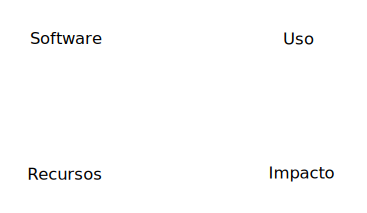
\includegraphics[scale=0.5]{imagens/process-model-scientific-software.png}
  \caption{A process model of software in science \cite{howison2015understanding}}
  \label{process-model-scientific-software}
\end{figure}

A Figura \ref{process-model-scientific-software} apresenta um diagrama deste
modelo de processo de softwares na ciência, este modelo é detalhado à seguir,
cada ator atua nos softwares, recursos, uso, impacto científico, detalhados à
seguir.

\subsection{Software}

Software acadêmico ({\it academic software}) é todo software usado para
coletar, processar ou analisar resultados de pesquisas com intenção de ser
publicados na literatura academica (seja num jornal, revista, conferência,
monografia, livro ou tese), podem ser desde protótipos escritos pelos próprios
cientistas, até mesmo produtos completos desenvolvidos profissionalmente
\cite{allen2017engineering}.

Podem ser encontrados na literatura acadêmica com outros nomes,
{\it research tool} \cite{Portillo12},
{\it research-originated software} \cite{Kon2011},
{\it research software} \cite{hettrick_2014_14809} ou
{\it scientific software} \cite{segal2008developing},
esses artefatos tem sido estudados dos mais variados pontos
de vista, desde de sua qualidade interna, até o impacto que
causam no meio científico.

No contexto de ecossistema de software acadêmico identificou-se cinco
motivações principais para a criação e contribuição ao software acadêmico:

\begin{enumerate}
  \item Ganho monetário direto (comercial software, employed software developers)
  \item Reputação acadêmica (incidental software, dirigido pela necessidade científica direta)
  \item Prática de software paralela (scientific needed enhanced by publishing 'software papers' alongside domain research)
  \item Um software de uma subárea de pesquisa (reputação direta pelo trabalho do software)
  \item Híbridos como licença-dual e 'software work' dentro de grandes colaborações (software como uma contribuição científica direta)
\end{enumerate}

\subsection{Recursos}

Os recursos investidos na produção destes softwares vem de diversas fontes,
incluem ganhos monetários diretos, recursos alocados em projetos, colaboração
entre laboratórios de pesquisa, e grande parte do ``tempo livre'' dos
pesquisadores em busca de soluções em suas pesquisas, este ``tempo livre''
perpassa por financiamentos diversos, carreira individual do cientista,
estudantes de graduação, prêmios, etc.

Independente da origem dos recursos o desenvolvimento de softwares acadêmicos
possui a particularidade de ser desenvolvido em sua grande maioria pelos
próprios cientistas uma vez que geralmente é necessário conhecimento no domínio
da pesquisa onde o software está inserido \cite{segal2008developing, hettrick_2014_14809,
momcheva2015software}.

\subsection{Uso}

% ... software é distribuido, utilizado e dá suporte à ciencia, gerando impacto ...

Estes artefatos de software são usados ativamente em diversos campos de pesquisa, como
matemática, biologia, física de partículas, astronomia, medicina e direito,
eles resolvem problemas comuns do cotidiano de pelo menos metade dos
pesquisadores de todas as áreas, desde grupos trabalhando exclusivamente com
problemas computacionais até grupos em laboratórios tradicionais ou em campo
\cite{wilson2014best}.

Os cientistas usuários finais mencionam tais softwares em suas publicações,
seja através de citação formal, informal, ou qualquer outro tipo de menção ao
software em suas pesquisas, estas citações ou menções fazem parte da economia
de reputação científica e causam impacto científico.

O impacto científico geralmente justifica o investimentos de novos recursos ao
ecossistema do software, seja para fins de planejamento, seja como
retrospectiva para avaliar os investimentos já realizados.

\subsection{Impacto científico}

% ... impacto científico justifica e potencialmente gera mais recurso ...
% \cite{katz2014transitive}

Ao longo da história, a citação formal tem sido utilizada para garantir
autenticação e autoridade, em vez de dar crédito e promover reconhecimento, na
história ocidental a citação aparece no final dos anos 1500, no início dos anos
1700 surge também no sistema legal, o ``copyright'' como reconhecendo aos
direitos autorais também surge nesse período, 1710.

A autoria das publicações tem sido realmente usado para reconhecer os autores e
contribuidores de um certo estudo, por exemplo, nos casos em que vários grupos
reivindicam crédito pelo mesmo avanço, ``backward citing'' tem sido utilizado
para verificar como as maiores comunidades de pesquisa atribuem crédito,
``forward citing'' também tem sido usada em casos onde se quer entender como
uma idéia foi usada após o seu surgimento ou publicação.

Conhecimento novo é claramente construído a partir do conhecimento passado.
Tradicionalmente, um autor cita um artigo anterior adicionando uma referência
ao autor, título, local de publicação, etc. No entanto, esse conceito não
funciona bem para produtos digitais como o software, que muitas vezes depende
de outros softwares, fragmentos de código, e algoritmos.

Este debate tem sido realizado a bastante tempo entre as diversas áreas da
bibliometria, cienciometria, altmetria e áreas similares, o fator de impacto
por exemplo proposto em 1955 apesar de continuar contribuindo para a ciência se
mostra muitas vezes utilizado da forma errada e mostra as deficiências de lidar
bem com produtos digitais gerados durante pesquisas.

\section{Sustentabilidade do ecossistema de software acadêmico}

% problemas identificados no ecossistema de software acadêmico

Um estudo sobre ecossistema de software acadêmico percebeu através dos relatos
de grande parte dos colaboradores participantes do estudo que os projetos de software
acadêmicos desenvolvidos na própria academia sofrem de {\it ``dysfunctional
chaotic churn''}, ou seja, a existência de muitos projetos, com poucos
usuários, com ciclos de vida curtos, que terminam em paralelo ao financiamento
inicial, comunidades desconectadas e paralelas, incompatibilidades entre
projetos, e tentativas aparentemente não coordenadas de ``reiniciar'' tudo
({\it re-boots}) \cite{howison2015understanding}.

Apesar de não haver evidências a respeito deste problema de forma tão abrangente,
sabe-se que parte dos problemas são realmente fato, por exemplo,
o {\it Dagstuhl Perspective Workshop}, evento organizado por um grupo de
pesquisadores sêniores de renome internacional, realizado anualmente na
universidade de Dagstuhl\footnote{\url{http://www.dagstuhl.de}} com o objetivo
refletir sobre o estado da ciência da computação explorando tópicos novos e
emergentes, em sua mais recente edição o workshop debateu sobre software
acadêmico e os problemas comuns em seu desenvolvimento, reconhecimento e
sustentabilidade \cite{allen2017engineering}.

\subsection{Desenvolvimento}

O desenvolvimento de software acadêmico ocorre em grande parte dentro da
própria academia, estudos mostram que pelo menos metade dos cientistas desenvolvem
seus próprios softwares, ao menos pacialmente, em domínios específicos este
número pode ser bem maior, na astronomia, por exemplo, estudos mostram que este
número pode chegar a 90\% \cite{hettrick_2014_14809, momcheva2015software}.

A grande participação dos cientistas no desenvolvimento destes artefatos de
software costuma ser um reflexo do tipo de conhecimento necessário ao se
desenvolver tais artefatos de software, pode ser necessário entender como o DNA
genômico se transforma em cristais de proteína, ou os meandros da dinâmica dos
fluidos, ou como resolver 20 equações diferenciais parciais simultâneas
\cite{segal2008developing}.

Desenvolvimento de software, exige algum conhecimento sobre o domínio, software
acadêmico não é diferente, mas esta grande participação dos cientistas no
desenvolvimento de software acadêmico começa a se tornar uma preocupação à
medida que a maior parte não possui treinamento algum sobre como escrever
softwares de forma eficiente, muitos não testam ou documentam os seus
softwares, faltam práticas básicas de desenvolvimento, como escrever código
legível, revisão de código, controle de versão, testes unitários, entre outros
\cite{wilson2017good}.

A qualidade dos softwares acadêmicos tem sido questionada,
a maioria também não sabe o quão confiável seu software é \cite{Merali2010Computational},
muitos estão em estado inicial de desenvolvimento \cite{marshall2013tools},
poucas foram testados fora do contexto onde foi desenvolvido \cite{Portillo12}.

Ocasionando sérios erros computacionais em conclusões centrais da literatura
acadêmica, gerando retrabalho para retratar tais erros nas mais diversas áreas
da ciência \cite{Merali2010Computational}. Dados são perdidos, análises levam
mais tempo que o necessário e os pesquisadores não conseguem a eficiência que
poderiam ter ao trabalhar com softwares acadêmicos \cite{wilson2017good}.
Causando um impacto negativo na visibilidade dos softwares acadêmicos
\cite{howison2013, katz2014transitive} e na capacidade de serem encontrados e
compartilhados.

\subsection{Reconhecimento}

% visibilidade

Apesar do crescimento no uso de software e na consequente dependência entre
cientistas de todos os campos, tornando o software acadêmico parte integral da
prática científica, apesar do apelo da comunidade científica para que o
software acadêmico seja tratado como cidadão de primeira classe, estudos tem
mostrado que muitas pesquisas não mencionam sequer o uso de software acadêmico
em suas publicações mesmo tendo feito uso de tais artefatos
\cite{momcheva2015software} \cite{howison2016software}.

Isto tem prejudicado a visibilidade do software acadêmico causando impacto
negativo em seu ecossistema, um software invisível é frequentemente excluído de
revisões por pares, uma atividade que costuma contribuir para a qualidade geral
do trabalho publicado, além disso, o
impacto negativo na visibilidade do software acadêmico faz surgir uma
série de questionamentos sobre a sua qualidade e também sobre a
capacidade de ser encontrado, compartilhado e co-desenvolvido
\cite{howison2013, katz2014transitive} \cite{howison2016software}.

Apesar de nem sempre ser possível, ou viável, ter tudo dentro de padrões
estritos, é preciso estar consciente das boas práticas ao produzir e utilizar
softwares acadêmicos, tanto para melhorar a própria abordagem quanto para
revisar outros trabalhos \cite{wilson2014best}.

Um software acadêmico em bom funcionamento devem atingir não apenas os
objetivos de entendimento e transparencia, mas também os objetivos voltados
para replicação \cite{Stodden2010}, seja logo após sua publicação, seja daqui
a 10 ou 50 anos.

\subsection{Sustentabilidade}

O desenvolvimento de software sustentável tem sido identificado como um desafio
chave no campo da ciência e da engenharia computacional, se sustentabilidade
não for levada em consideração em projetos de software, não importa qual o
domínio ou qual o propósito do software, perde-se a oportunidade de causar
mudanças positivas no planeta e na sociedade.

Apesar de sustentabilidade ser um conceito complexo e com mútiplas dimensões,
levando a debates profundos, o conceito geral é bastante simples e refe-se à
capacidade de perdurar e de continuar sendo suportado ao longo do tempo, isto
implica na qualidade de longevidade e manunetabilidade do software
\cite{venters2014software}.

Software sustentável é aquele que continua a estar disponível no futuro, em
novas plataformas, atendendo continuamente às novas necessidades do ambiente
... adequada evolução frente as condições do ambiente em constante mudança
\cite{allen2017engineering}.

Estudo mostra o decaimento das URLs ao longo do tempo, fundamenta o assunto,
mostra grafico com o caimento ao longo dos anos em publicações da
bioinformática, grafico muito bom cruzando e decaimento e tendencia com os
passar do tempo \cite{wren2017use}.

O {\it Journal of the American Statistical Association (JASA)} tem insistido na
necessiade de estarem disponíveis código e dados durante a revisão dos
manuscritos \cite{baker2016scientists}, Agências de financiamento como o {\it
US National Science Foundation} estão começando a reconhecer produtos de
pesquisa, como software, assim como fazem com as publicações, isto reconhece as
contribuições ao softwares assim como primeiro produto de pesquisa.

Isto visa especialmente garantir a longevidade dos artefatos e proporcionar que
um segundo pesquisador receba todos os benefícios do trabalho duro do primeiro
pesquisador \cite{king1995replication}, já que tanto a ciência quanto a
engenharia dependem de resultados incrementais para sua evolução. No terceiro
compromisso, relacionado ao conceito {\it desenvolvimento}, o Dagstuhl
Manifesto enfatiza a necessidade de medir a qualidade e a sustentabilidade dos
softwares científicos, tanto a priori quanto a posteriori.

\subsubsection{Manutenabilidade}

% falar de manutenabilidade como um eixo dentro de sustentabilidade técnica

A adoção e uso de softwares acadêmicos está relacionada, entre outros fatores,
também à sua qualidade, portanto é impoprtante medir e coletar sua qualidade de
alguma forma, qualidade é um vasto assunto, um dos problemas comuns enfrentado
pelos pesquisadores que desenvolvem tais softwares é a manutenabilidade
\cite{Prlic2012}.

Estudos tem mostrado que grande parte das ferramentas de software criadas na
academia estão em estado inicial de desenvolvimento \cite{marshall2013tools} e
que apenas uma pequena porcentagem são testados fora do contexto onde foi
desenvolvido \cite{Portillo12}.

%%%%%%%%%%%%%%%%%%%%%%%%%%%%%%%%%%%%%%%%%%%%%%%%%%%%%%%%%%%%%%%%%%%%%

%Cita um mapeamento feito sobre estudos que criam ferramentas para apoio a
%revisão sistemática no domínio de SE, 14 estudos foram selecionados, ao final
%apenas 8 tinham proposta de ferramentas, ao final conclui que as ferramentas
%encontradas estão em estado inicial de desenvolvimento \cite{marshall2013tools}.

%Cita um mapeamento sistemático com objetivo de encontrar ferramentas de
%comunicação e coordenação para suporte a times altamente distribuidos
%gograficamente, encontrou 132 ferramentas, para uso em projetos de software
%global. A maioria destas ferramentas foram desenvolvidas em centros de
%pesquisas, e apenas uma pequena porcentagem (18.9\%) foram testados fora do
%seu contexto onde foi desenvolvido \cite{Portillo12}.

%Computer systems research spans sub-disciplines that in-
%clude embedded and real-time systems, compilers, network-
%ing, and operating systems. Our contention is that a number
%of structural factors inhibit quality research. We highlight
%some of the factors we have encountered in our work and ob-
%served in published papers and propose solutions that could
%both increase the productivity of researchers and the quality
%of their output \cite{Vitek2011}.

%Além da aplicação, estes softwares variam também no papel que ocupam em suas
%pesquisas, alguns fazem parte dos resultados da pesquisa, como por exemplo,
%propostas de novos algoritmos ou técnicas de produção, outros são utilizados
%como parte do método de pesquisa, como coleta ou análise de dados, sendo que
%estes papeis não são excludentes.
%
%estes costumam ser citados pelos seus autores como uma das contribuições do
%estudo, seja principal ou secundária, 
%Esses softwares podem, de fato, ser um software de simulação complexo desenvolvido
%e executado em um computador de alto desempenho, mas também pode ser um
%software desenvolvido em um PC para incorporação em instrumentos; para
%manipular, analisar ou visualizar dados; ou para orquestrar fluxos de trabalho.

%e à medida
%que percebe-se que os softwares estão se tornando parte integrante dos
%processos, ferramentas e produção científicas, torna-se necessário e urgente
%discutir o seu desenvolvimento, visibilidade, qualidade e sustentabilidade.

% mostrar os beneficios da ciencia aberta, ciberinfraestrutura, etc
% * (favorecendo a ciencia e tornando a vida mais feliz para todos)

% mostrar os problemas para a ciência como um todo
% * causando problemas para o progresso de ciência, dados perdidos, etc, retrabalho
%   dificuldade de reprodução, etc...

%, não apenas técnica, mas também a
%capacidade de ser encontrado, compartilhado e co-desenvolvido, qualidades
%importantes para a evolução do próprio software, mas também extremamente útil
%para um uso eficiente dos limitados recursos da ciência \cite{howison2013,
%katz2014transitive}.

%contradizendo as boas
%práticas de qualquer projeto experimental, de ter {\it laboratory
%notebooks}\footnote{\url{https://en.wikipedia.org/wiki/Lab_notebook}}, dados
%organizados, passos documentados, e projeto estruturado para reprodutibilidade.

%softwares acadêmicos, assim
%como qualquer outro aparato experimental, são tão importantes para a ciência
%quanto são os telescópios ou tubos de ensaio \cite{wilson2014best}.

%Cientistas gastam mais tempo hoje utilizando e desenvolvendo softwares do que
%gastavam no passado.

%Software is a critical part of modern research and yet there is little support across the
%scholarly ecosystem for its acknowledgement and citation. Inspired by the activities
%of the FORCE11 working group focused on data citation, this document
%summarizes the recommendations of the FORCE11 Software Citation Working
%Group and its activities between June 2015 and April 2016. Based on a review of
%existing community practices, the goal of the working group was to produce a
%consolidated set of citation principles that may encourage broad adoption of a
%consistent policy for software citation across disciplines and venues. Our work is
%presented here as a set of software citation principles, a discussion of the motivations
%for developing the principles, reviews of existing community practice, and a
%discussion of the requirements these principles would place upon different
%stakeholders. Working examples and possible technical solutions for how these
%principles can be implemented will be discussed in a separate paper.
%\cite{smith2016software}

%Improving academic software engineering projects: A comparative study of academic and industry projects
%(compara as praticas de desenvolvimento da industria e academia e sugere melhorias, 1998!)
%https://link.springer.com/article/10.1023%2FA%3A1018925902814?LI=true

% papel pesquisador no ecossistema de soft academico
%
%Essas preocupações gerais sugerem um conjunto de questões específicas, com foco
%em padrões globais e padrões emergentes dentro do ecossistema, incluindo: Quais
%recursos foram destinados à produção de software? Quantos usuários ou
%comunidades de usuários têm projetos? Quais são os impactos científicos desse
%uso? Os números de usuários crescem? Os projetos possuem recursos e habilidades
%suficientes para gerenciar seu crescimento? Quais projetos possuem
%funcionalidades sobrepostas? Há quanto tempo os pedaços de software e projetos
%persistem? Nós desconectamos as comunidades de usuários e desenvolvedores? São
%componentes específicos, ou camadas de componentes, faltam? Que código
%geralmente é usado em conjunto; são os projetos e as pessoas que produzem esses
%componentes se comunicando adequadamente? Como podemos sustentar o software
%crítico?
%
%Aqui há uma clara tensão entre um desejo de flexibilidade e liberdade, ligado
%às expectativas de inovação científica e desejos de estruturas de autoridade e
%controle de coordenação. As questões de influência incluem: como os programas
%de financiamento e quais os requisitos em suas chamadas, resultaram em software
%amplamente utilizado e impacto científico substancial? Quais são as
%características dos campos que alcançaram maior coalescência? Quais jornais e
%conferências têm políticas exemplares? Como o trabalho de software é visto
%dentro das práticas de contratação e avaliação, como os casos de posse?
%
%\cite{howison2015understanding}

%Ao longo da história, a citação formal foi para autenticação e autoridade, em
%vez de de crédito e reconhecimento ou atribuição. A  científico citação na
%história ocidental aparece no final dos anos 1500. No início dos anos 1700, a
%citação também aparece no sistema legal como método de compreensão dos
%precedentes \cite{katz2014transitive}.

%A ideia de direitos autorais como reconhecendo aos direitos dos seus autores
%também surge nesse tempo, 1710, talvez devido a uma lenta tendência social
%societária de reconhecer a propriedade intelectual, uma idéia que parece ter se
%desenvolvido ao lado da imprensa]. Observe que a autoria de papers é realmente
%usado para notar os autores reais do artigo quanto para notar os contribuidores
%do projeto.
%Para muitos desses, o
%identificador que deve ser citado - um "nome" que se refere a um produto único
%não é claro.

%Additionally, if a cited library depends
%on another library, the contribution of this second library
%is not captured. Citation of a dataset should perhaps give
%credit to the people who gathered the data, as well as
%those who curated it, but the paper author may not know
%or be able to find these details.

%Mas independente de como seja calculado o impacto científico de uma determinada
%pesquisa o impacto causado se reverte potencialmente em mais recursos que
%poderão ser reinvestidos no próprio ecossistema onde o software está inserido.

%Science Code Manifesto \cite{barnes2013science}.
%Foco em código fonte escrito especificamente para processar dados de
%publicações, afirma que ``todo código fonte escrito especificamente para
%processar dados de uma publicação deve estar disponível para os revisores e
%leitores do paper''.

%Sustentabilidade é um conceito guarda chuva composto de múltiplas dimensões, em
%sua dimensão técnica, chamada sustentabilidade técnica, temos a preocupação com
%a longevidade da informação, dos sistemas, e infraestrutura, e sua adequada
%evolução frente as condições do ambiente em constante mudança.

%citações formais facilitam e promovem o avanço
%da ciência, mesmo diante da falta de um padrão para citar artefatos digitais
%\cite{allen2014credit}.

%Um estudo recente com 90 artigos de diversas áreas da biologia, selecionados
%aleatoriamente entre publicações usando softwares como método, mostrou que
%apenas 59 mencionavam o uso de softwares de alguma forma, os demais 31 artigos,
%apesar de usar software acadêmico, não mencionavam nada a respeito
%\cite{howison2016software}, apenas entre 31\% e 43\% das menções aos softwares
%acadêmicos envolvem citação formal.

%Não existe ainda amadurecimento suficiente sobre como citar softwares e
%outros artefatos digitais em pesquisas científicas, não temos um padrão de como fazê-lo,
%cada autor cita à sua maneira, muitas vezes ao longo do texto, outras em seções
%específicas sobre a implementação do software, nem semprem informam onde
%encontrar uma cópia do software, ou ainda nem sobre o modelo em que o software
%é distribuído, ou se é de alguma forma distribuído ao público.

%Entre os softwares acadêmicos desenvolvidos por cientistas como apoio em suas
%pesquisas, não é raro que pesquisadores deixem de disponibilizar estes artefatos,
%assim como outros desdobramentos da pesquisa, como dados e outros. Ou ainda,
%mesmo disponibilizando tais artefatos em locais de público acesso, com o tempo,
%tais locais se tornam indisponíveis inviabilizando a obtenção de tais
%artefatos.

%A comunidade tem refletido sobre os problemas relacionados ao
%desenvolvimento, promoção e sustentabilidade desses softwares, e o
%impacto que tais problemas causam no meio científico \cite{allen2017engineering}.

%, e faz
%surgir questionamentos sobre sua qualidade, não apenas técnica, mas também a
%capacidade de ser encontrado, compartilhado e co-desenvolvido, qualidades
%importantes para a evolução do próprio software, mas também extremamente úteis
%para o uso eficiente dos limitados recursos da ciência \cite{howison2013,
%katz2014transitive}.

\section{Ecossistema de software acadêmico de análise estática} \label{analise-estatica}

Ao falarmos sobre ecossistema de software acadêmico estamos nos referindo a
qualquer software, de qualquer domínio de aplicação, que tenha sido utilizado
ou produzido durante trabalhos de pesquisa com intuito de publicação na
literatura acadêmica.
%REVER - intuito de apoiar pesquisa que será eventualmente divulgada por meio da  publicação de resultados.

O ecossistema de software acadêmico de análise estática é um recorte deste
conjunto, a princípio, com as mesmas características, atores e modelo de
funcionamento, mas logicamente podendo apresentar particularidades trazidas
pela natureza do domínio de análise estática e suas ferramentas, soluções e
algoritmos.

\subsection{Análise estática}

A análise estática de código fonte é o primeiro passo para coletar informações
necessárias em diversas atividades de verificação, medição e melhoria da
qualidade de produtos de software \cite{cruz2009code, kirkov2010source}. Ela é
realizada com base no código fonte de um programa ou sistema de software, e a
partir daí descobre problemas e propriedades de sua qualidade estrutural
\cite{chess2007secure}.

Ferramentas de análise estática estão disponíveis há décadas, em especial,
para programadores. A ferramenta Lint \cite{johnson1978lint}, considerada a
primeira ferramenta de análise estática \cite{gosain2015static}, foi criada para
examinar programas escritos em linguagem C e aplicar regras de tipagem mais
estritas do que as regras dos próprios compiladores da linguagem.

Análise estática de código fonte tem como objetivo prover
informações acerca de um programa a partir do seu código fonte sem
necessidade de execução, e sem requerer qualquer outro artefato do programa
além do próprio código.

É um ramo que possui muitas das suas abordagens em comum com os estudos da
área de análise de programas ({\it program analysis}), especialmente na área de
compiladores, onde atua especialmente nas primeiras etapas do processo de compilação.

A análise estática de código fonte é considerada uma atividade meio com
objetivo de suportar uma variedade de tarefas comuns da engenharia de
software; muitas dessas tarefas são substancialmente úteis em atividades de
manutenção, incluindo \cite{binkley2007source}:

\begin{multicols}{2}
  \begin{itemize}
    \item Análise de performance
    \item Compreensão de programas
    \item Desenvolvimento baseado em modelos
    \item Detecção de clones
    \item Evolução de software
    \item Garantia de qualidade
    \item Localizaçao de falhas
    \item Manutenção de software
    \item Recuperação arquitetural
    \item Testes
  \end{itemize}
\end{multicols}

Seja em qual atividade for, a análise estática possui importância,
pois ao ser capaz de extrair informações diretamente do
código fonte de um programa, pode auxiliar a responder perguntas necessárias
para as diversas atividades de desenvolvimento e evolução de software. Essa
importância se torna ainda mais aparente diante da ``lei'' da tendência para
execução \cite{harman2010why} que indica que todos os tipos de notação tem a
tendência de se tornar executáveis.

% \subsection{Usos da análise estática de código fonte} \label{usos}

A análise de programas trata, de modo geral, da descoberta de problemas e
fatos sobre programas. Tal análise pode ser realizada sem a necessidade de executar o
programa (análise estática) ou com informações provenientes de sua execução
(análise dinâmica).

A ideia de que programas de computador podem ser utilizados para analisar
código fonte de outros programas tem uma história de mais de 40 anos.  O
programa PFORT \cite{ryder1974pfort} foi projetado para localizar potenciais
problemas na portabilidade de código Fortran; em função da diversidade de
dialetos de Fortran, uma compilação sem erros não indicava que o programa
estava correto segundo os padrões da linguagem \cite{wichmann1995industrial}.

Desde então, ferramentas de análise estática de código fonte têm surgido para
os mais diversos fins -- muitas delas a partir das pesquisas e
desenvolvimentos da área de compiladores.  O {\it parser} utilizado nessas
ferramentas têm funcionalidades análogas aos analisadores usados em
compiladores \cite{anderson2008the}.

O uso de tais ferramentas tem se tornado mais comum no ciclo de desenvolvimento de
software, sendo aplicadas em atividades distintas.
O campo de aplicação destas ferramentas é bastante variado, cobrindo diferentes
objetivos.

\subsection{Software de análise estática}

A variedade de aplicação e a constante evolução da área de análise estática, 
tanto na indústria quando na academia, resulta em  estudos teóricos e práticos, novas ferramentas, modelos e
algoritmos de análise estática. Ferramentas de análise estática têm sido
continuamente desenvolvidas e seu uso se tornado comum no ciclo de desenvolvimento de
software.

Mas apesar da rápida e constante evolução da área, ainda há carência de estudos
avaliando estas ferramentas \cite{li2010comparative}, mesmo com os avanços e com
ferramentas de sucesso, o desenvolvimento de análise estática ainda é conhecido
por ser um processo doloroso \cite{toman2017taming}.

A eficiência, confiabilidade e precisão dessas ferramentas têm sido avaliadas e
alguns estudos mostram inconsistência entre ferramentas diferentes.
Um estudo que comparou duas ferramentas de análise estática para cálculo de métricas,
revelou significantes evidências sobre a inconsistencia entre valores de métricas,
grande diferença nos valores, e discutiu quais problemas e questões levam a estas
diferenças \cite{alemerien2013experimental}.

Análise estática é a técnica mais amplamente utilizada para análise
automatizada de programas devido a sua eficiência, boa cobertura e automação.
Estudos mostram que analise estática tem grande adoção em projetos de software
livre \cite{beller2016analyzing}.
Entretanto,tecnicas de analise estatica amplamente adotadas na comunidade de software,
por exemplo, para localização de bugs e verificação de programas 
ainda sofrem um alto índice de falso-positivos \cite{gosain2015static}.

Apesar da ampla adoção de ferramentas de análise estática em estudos
acadêmicos e da crescente atenção que as técnicas de análise estática de código tem
recebido em pesquisas, nota-se ainda uma enorme distância entre a atenção dada na academia e sua adoção na indústria,
identificando um gap entre estes dois contextos \cite{ilyas2016static}.

\subsection{Software acadêmico de análise estática}

Em Ciência da Computação, particularmente em Engenharia de Software, tem-se
notado um aumento constante no número de novos softwares acadêmicos \cite{allen2017engineering},
especialmente em estudos de análise estática, 
uma área com uma longa e respeitável tradição em
pesquisas sobre a criação de novas ferramentas, métodos e algoritmos.

%Na indústria também a adoção de software de análise estática é crescente...

O software acadêmico de análise estática e o seu ecossistema, ao estar inserido
no sistema acadêmico e intimamente relacionado a economia de reputação
científica, sofre as consequências da competição que permeia este modelo, e o
seu uso invariavelmente deixa de gerar feedback positivo de volta ao seu ecossistema,
conforme Figura \ref{scientific-reputation-diagram}, onde se apresenta o
relacionamento entre a prática e a pesquisa de software acadêmico.

%está inserido no contexto similar
%a qualquer outro software acadêmico, e o seu ecossistema possui as mesmas
%características do ecossistema de software acadêmico, 

\begin{figure}[h]
  \center
  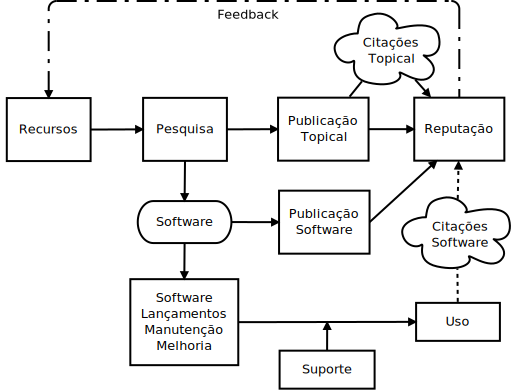
\includegraphics[scale=0.5]{imagens/scientific-reputation-diagram.png}
  \caption{Uma visão dos incentivos de reputação num contexto misto entre Ciência e práticas de software acadêmico \cite{howison2011scientific}}
  \label{scientific-reputation-diagram}
\end{figure}

%ecossistema de software acadêmico está inserido num contexto de competição

Diferentemente de outras tecnologias, software pode ser copiado e distriduído
essencialmente sem custo, abrindo portas sem precedentes em nível para
compartilhamento e inovação colaborativa \cite{howison2011scientific}, no
entanto, ao estar de alguma forma conectado ao contexto de competição da economia de
reputação científica, como no mecanismo de crédito acadêmico aos artigos e publicações,
pode ser potencialmente problemático para a colaboração e manutenção
\cite{howison2011scientific}.

%No entanto tem se percebido que o ecossistema de software acadêmico tem perdido
%oportunidade de colaboração visto que estão inseridos neste contexto ....
%competição, muitos softwares utilizados em pesquisas não são mencionados pelos
%seus autores causando impacto negativo em sua visibilidade, reconhecimento e
%consequentemente ...  \cite{howison2016software}.

Este cenário, além de desacelerar o progresso geral da Ciência gerando
retrabalho, faz surgir questionamentos sobre as conclusões dessas pesquisas,
especialmente quando grande parte dos pesquisadores não sabem o quão confiável
seus projetos de software são. Criando assim, um contexto em que muitos estudos
em Engenharia de Software sofrem de dificuldades de repetição
\cite{tang2016worthiness}, além de ocasionar problemas específicos relacionados a
manutenabilidade e sustentabilidade técnica do software acadêmico.

%Esta reflexão tem mostrado,
%por exemplo, 

%Junto com estas questões estão as questões de como
%influenciar o ecossistema, incluindo questões de pontos de inflexão que levam
%ao uso coalescente, bem como a intervenções políticas diretas incentivando o
%uso de componentes específicos.

%%%%%%%%%%%%%%%%%%%%%%%%%%%%%%%%%%%%%%%%%%%%%%%%%%%%%%%%%%%%%%

%While some of these seem relatively unproblematic, such as commercial
%production in fields with immediately valuable applications, others appear
%problematic. In particular we highlighted the potentially pernicious
%implications of the academic credit production system for collaboration and
%maintenance 

%Adicionalmente as relacões entre os atores do ecosistema como um todo
%são de mútuo interesse (mutualismo):

%O relacionamento entre os atores em um ecossistema de software, por outro lado,
%são caracterizados pela alto espectro de relacionamentos simbioticos.

%Dependendo dos atores e suas atividades, dois atores podem ter benefícios
%mútuos (mutualismo), estar em competição direta (competition/antagonism),
%estarem não afetados (neutralism) ou um não afetado enquanto o outro é
%beneficiado (amensalism) ou prejudicado (parasitism) por seu relacionamento

%em pesquisas sobre análise de código, ferramentas de analise estatica tem
%recebido significante mais atencao que outras tecnicas, tecnicas com formal e
%bem definidos processos recebem mais atencao de pesquisa e escrutinio porque
%estudos irao avaliar seu processo e elementos, entretanto, isto nao
%necessariamente significa que tecnica é melhor; The survey concluded that 1)
%the adoption of static code analysis techniques in the industry is influenced
%by the software life cycle model, while software product type and company size
%doesn’t have an influence. 2) The amount of attention a static code analysis
%technique has received in research doesn’t necessarily influence its adoption
%in industry indicating a gap between research and industry 3) company size,
%product type, and life cycle model do influence professionals perception on
%benefits/limitations.  \cite{ilyas2016static}

\section{Ciência e colaboração}

\subsection{Reprodutibilidade}

Enquanto pesquisadores publicam artigos descrevendo e divulgando seus
resultados, é raro que façam o mesmo com toda a produção gerada durante a
pesquisa. A maioria dos componentes necessários para a reprodução dos
resultados de uma pesquisa -- por exemplo, códigos fonte e dados -- usualmente
permanecem não publicados. Esse problema fere um dos fundamentos
da ciência de que novas descobertas sejam reproduzidas antes de serem
consideradas parte da base de conhecimento \cite{Stodden2009}.

%Nesse sentido, \citeonline{Prlic2012} enfatizam que disponibilizar o código
%criado durante pesquisas não apenas aumenta o impacto como também se torna
%essencial para outros reproduzirem os resultados encontrados, citam ainda que
%manutenabilidade e disponibilidade do software após a publicação é o maior
%problema enfrentado pelos pesquisadores que desenvolvem tais softwares.
%
%A replicação desses estudos empíricos pode, e deve, ser realizado, de modo a
%averiguar a validade e aumentar o nível de confiança em seus resultados,
%replicação costuma ser citado como um importante meio para validar estudos
%empíricos e assim aumentar o nível de confiança em seus resultados
%\cite{Almqvist2006}. A reprodução dos resultados de pesquisas aumenta o impacto
%social das pesquisas e gera economia de tempo e dinheiro para os pesquisadores
%e para as instituições \cite{Nesta2010}.

Apesar da preocupação com a reprodutibilidade dos resultados de pesquisas de
forma independente \cite{Stodden2009} e aberta, esta área tem recebido ainda
pouca atenção da comunidade de pesquisa \cite{Nancy2015, Grand2010Open}. Em um
estudo recente, com 88 papers do MSR entre 2004-2011, evidenticou-se que apenas
62\% são replicaveis ou parcialmente replicaveis e que apenas 20\% dos estudos
disponibilizam suas ferramentas \cite{amann2015software}. Um estudo anterior
com 171 papers do MSR evidenciam que, entre outros problemas, a maioria não
disponibilizam publicamente as ferramentas e scripts, mesmo quando os autores
explicitamente afirmam que construíram algum \cite{robles2010replicating},
apenas 2 entre 154 estudos experimentais avaliados fornecem os dados e as
ferramentas necessárias para replicação e futuras pesquisas
\cite{barr2010shoulders}.

Reprodutibilidade ({\it reproducibility}) é a habilidade de replicar um experimento
ou estudo em sua totalidade a fim de confirmar suas hipóteses, seja pelo
autor ou por pesquisadores independentes. Esse conceito é um ponto
central do método científico e continua a receber bastante atenção ainda hoje,
como pode ser verificado em estudos recentes.

\citeonline{Stodden2009} preocupada com as barreiras legais para
disponibilidade de artefatos de pesquisa propõe o framework ``{\it Reproducible
Research Standard (RRS)}'', onde sugere formas de usar o licenciamento e as leis
de copyright da melhor forma para manter disponíveis os produtos gerados
durante pesquisas e assim viabilizar reprodutibilidade. \citeonline{Vitek2011}
em um estudo sobre reprodutibilidade e rigor científico destacam a importancia
de se disponibilizar qualquer material suplementar gerado durante uma pesquisa
de modo a possibilitar revisores verificarem e replicarem experimentos. Em
2012, um workshop intitulado ``{\it Reproducible Research: Tools and Strategies for
Scientific Computing}'' \cite{Stodden2012} discutiu, especificamente, iniciativas
e ferramentas voltadas a apoiar pesquisas reprodutíveis.
\citeonline{Krishnamurthi2015}, em um estudo sobre repetibilidade, chamam
atenção para o papel central que os artefatos de software possuem em pesquisas
de ciência da computação e questionam: "Onde está o software nas pesquisas
sobre linguagem de programação?". \citeonline{Stodden2015} demonstram o
projeto "ResearchCompendia.org", uma infraestrtura para reprodutibilidade e
colaboração em ciência computacional. Além destes e tantos outros estudos em
\cite{GithubReproducibilityGuide} é possível acessar um guia sobre como
desenvolver pesquisas cientíticas de forma que promovam a reprodutibilidade.

Apesar do termo reprodutibilidade ser relativamente concensual entre as várias
áreas da ciência, existem alguns termos relacionados com uma certa diferença
de significado, diante disto, e preocupado em criar uma linguagem comum entre
os pesquisadores, \citeonline{Feitelson2015} propôs as seguintes definições:

\begin{description}

  \item[Repetição (repetition)]
  Refazer exatamente o que outra pessoa fez usando os artefatos originais.

  \item[Replicação (replication)]
  Replicar com precisão exatamente o que outra pessoa fez, recriando os
  artefatos.

  \item[Variação (variation)]
  Repetir ou replicar exatamente o que a outra pessoa fez, mas com alguma
  modificação controlada nos parâmetros.

  \item[Reprodução (reproduction)]
  Recriar o espírito do que outra pessoa fez, usando seus próprios artefatos.

  \item[Corroboração (corroboration)]
  Obter os mesmos resultados de outra pessoa, usando outros meios e
  procedimentos experimentais.

\end{description}

É conhecido que a ciência precisa de reprodutibilidade e corroboração para
realmente fazer progressos, mas a prática de forma abrangente ainda é um
obstáculo. Diante disso \citeonline{Peng2011} sugere adotar soluções
intermediárias, repetição, replicação, variação, e desta forma já teríamos uma
grande melhoria sobre a situação atual onde muitos estudos em engenharia de
software sofrem de dificuldades de repetição \cite{Tang2016} e,
consequentemente, poucos estudos replicando pesquisas da área são encontrados
\cite{da2011replication}.

Mesmo sabendo que todo artefato tem impacto na reprodutibilidade
\cite{gonzalez2012reproducibility}, uma barreira comum para tal prática, e
consequentemente para repetição, replicação e variação é a indisponibilidade do
código fonte. Toda pesquisa que possua qualquer processo computadorizado deve
publicar seus códigos, eles precisam estar disponíveis, mesmo que os dados
correspondentes não estejam, o código deve estar. De acordo com o espectro de
reprodutibilidade (Figura \ref{reproducibility-spectrum}), a disponibilidade de
código é o requisito mínimo e é o primeiro passo para possibilitar validação e
confirmação dos resultados.

\begin{figure}[h]
  \center
  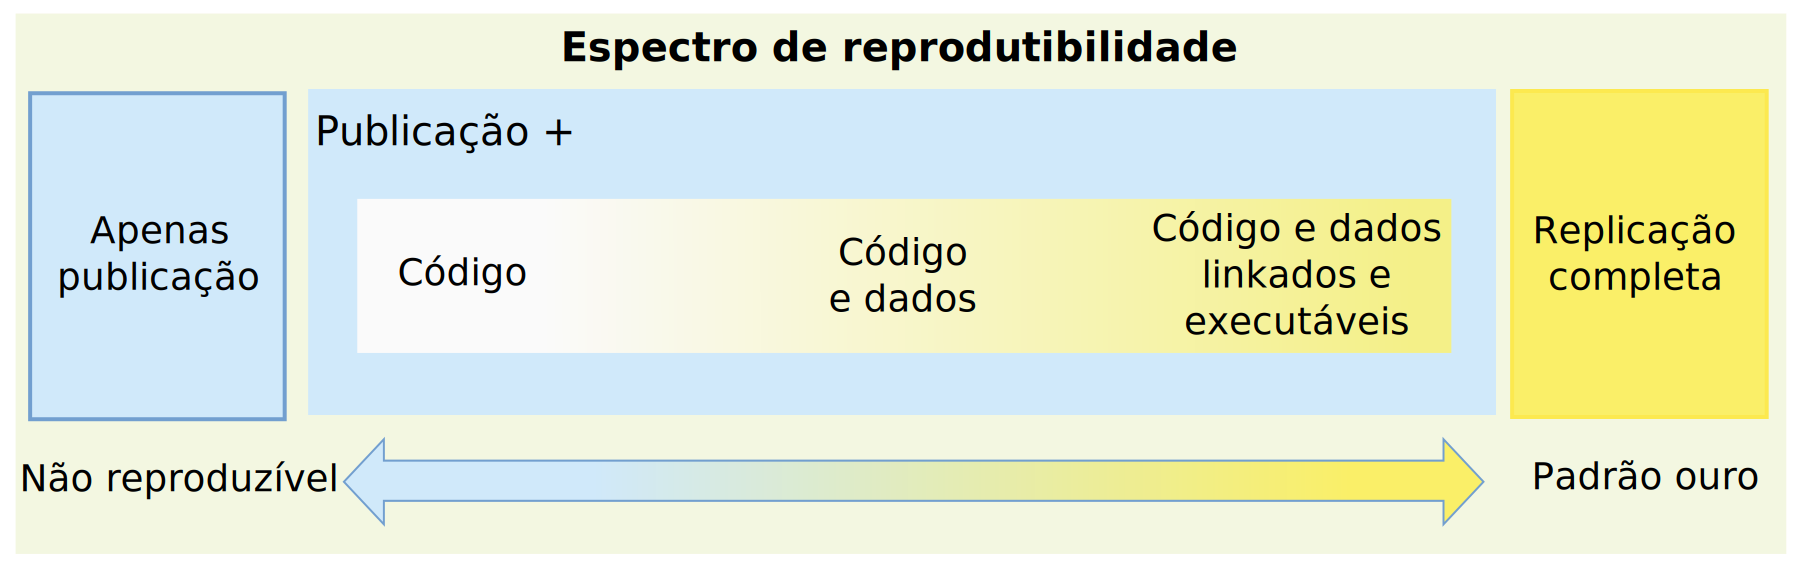
\includegraphics[scale=0.35]{imagens/reproducibility-spectrum-ptbr.png}
  \caption{Espectro de reprodutibilidade \cite{Peng2011}}
  \label{reproducibility-spectrum}
\end{figure}

Apesar das pesquisas reproduzíveis ({\it RR - Reproducible Research}) não
resolverem todos os problemas de validade experimental dos estudos em
engenharia de software, elas ao menos garantem que dados e métodos de análise
estejam disponíveis para inspeção e que os resultados possam ser derivados,
facilitando revisão logo que a publicação acontece. Além disso, é um recurso
valoroso para pesquisadores iniciantes, pesquisas reproduzíveis melhoram o
impacto do próprio estudo, por exemplo, artigos de computação que não
disponibilizam pubicamente dados e códigos possuem menos chances de serem
citados \cite{madeyski2017would}.

\subsection{Ciência aberta}

Ciência Aberta é um movimento que tem por objetivo tornar a pesquisa
científica, seus dados e sua disseminação acessíveis à todos os interessados,
sejam amadores ou profissionais \cite{WikipediaOpenScience}. Sua principal
motivação está em possibilitar a reprodução dos resultados de pesquisas e em
garantir transparência das metodologias utilizadas, isto aumenta o impacto
social das pesquisas e gera economia de tempo e dinheiro para os pesquisadores
e para as instituições \cite{Nesta2010}.

Este movimento é guiado por princípios básicos de transparência, acessibilidade
e reusabilidade universais, disseminadas via ferramentas online, ele é dividido
em quatro grandes áreas: (1) Open Access, (2) Open Data, (3) Open Source e (4)
Open Reproducible Research. Dentre elas destaca-se a Open Reproducible Research
por preocupar-se com a reprodutibilidade dos resultados de pesquisas de forma
independente \cite{Stodden2009} e aberta, no entanto, esta área tem recebido
ainda pouca atenção da comunidade de pesquisa \cite{Nancy2015}
\cite{Grand2010Open} apesar do aumento geral do interesse pelas práticas da
Ciência Aberta \cite{Grand2010}.

%Over the past fifteen years the scholarly communications agenda
%has progressed gradually. Currently we are experiencing a strong
%tendency among all research stakeholders to engage with the
%practice of OS. Lately, research funders require the sharing not
%only of the research results they have funded, but also of the
%procedures and data that are being generated during the research
%conduct. Researchers, on the other side, are keen on observing
%their research results being used for the improvement of the
%society and are forced by their funders to demonstrate the impact
%of their research. At the same time, higher academic institutions
%aim to join the OS agenda as well, since they see the opportunity
%of great economic benefits and savings. While OS is the possible
%answer to all these factors, the stakeholders’ inability to
%understand the requirements for the application of OS can be a
%suspensory factor for the OS implementation and evolution.
%The aim of the FOSTER project is to advance the stakeholders'
%knowledge on the usefulness of OS and explain the technicalities,
%strategies and best practices using which OS can be applied. As an
%attempt to educate the largest number of researchers possible,
%FOSTER has created an e-leanring portal, which contains quality
%assured information relating to the topic and it is open to everyone
%in the world. The platform contains two types of information:
%learning material and online courses. The classification of these
%two types is supported by an OS taxonomy, where related terms
%are applied both in the portal's material and also in the courses.
%With the use of the taxonomy, users are in the position to
%understand the OS domain and the concepts around it.
%The main goal of the FOSTER project, which is mainly achieved
%through the portal functionalities, is not only to educate the
%research stakeholders on OS, but also to build a community of
%researchers, librarians, software developers, funders and research
%administrators who are interested in OS in order to advance the
%way research is being conducted and shared. In addition, FOSTER
%attempts to provide tools to this community, such as re-usable
%content for training and a platform for blended learning and e-
%learning courses that the community could run. This OS
%advancement is essential for the research promotion and,
%consequently, for the benefit of the society as a whole
%\cite{Nancy2015}.
%
%Open Science may be practised both
%for philosophical and pragmatic reasons. As the
%resources produced by open projects are
%potentially accessible to public audiences, Open
%Science offers both a novel medium for public
%access and involvement in the process of science
%and an innovative method for real-time science
%communication. Does such direct access clear
%the stream of communication or muddy the
%waters with unfocussed, unclear and unvetted
%comment? This paper suggests that adopting an
%Open Science approach allows the capture of an
%authentic and clear record of research.
%However, researchers acknowledge this involves
%opening their work up to a different type of
%scrutiny \cite{Grand2010}.
%
%Open Science is an emerging approach to the conduct of science, technology and engineering
%projects, in which information about the whole of an ongoing investigation is made available
%on and through the Internet. Adopting an Open Science approach means the audience for the
%research can extend beyond the researchers involved to other researchers and to members of
%the public. Thus, Open Science has implications for engineering research, practice,
%publishing and public engagement with engineering. This paper reviews the history and
%evolution of the Open Science movement, includes some reflections on the related areas of
%Open Access, peer-review and public engagement with science and engineering and discusses
%data gathered from interviews. The analysis suggests that interviewees have concerns about
%issues such as precedence and protection of original work and the time needed to integrate
%open science practices into daily work. Successfully working in such collaborations is likely
%to require not only common practical tools but also the development of shared language and
%understanding between researchers and members of the public. Interviewees recognise the
%value of Open Science in collaborative research and its innovative facility to sustain direct
%public access to research outputs. It also has the potential to allow members of the public to
%make real practical contributions to research \cite{Grand2010Open}.
%
%This white paper was written as a contribution to the “Imagining
%Tomorrow’s University: Rethinking scholarship, education, and institu-
%tions for an open, networked era” workshop, a joint NIH/NSF-funded
%event held 8–9 March 2017 in Rosemont, IL. In this paper, I present an
%overview of what I consider open science, its importance, and how it
%plays a role in my research agenda. I also discuss challenges faced in
%pursuing research openness, and recommend changes to university
%leaders to address these barriers \cite{niemeyer2017open}.
%
%Open to All?  Case studies of openness in research
%Since the early 1990s, the open access movement has promoted the concept of openness in relation
%to scientific research. Focusing initially upon the records of science in the form of the text of articles
%in scholarly journals, interest has broadened in the last decade to include a much wider range of
%materials produced by researchers. At the same time, concepts of openness and access have also
%developed to include various kinds of use, by machines as well as humans.
%Academic bodies, including funders and groups of researchers, have set out statements in support
%of various levels of openness in research. Such statements often focus upon two key dimensions:
%what is made open, and how; and to whom is it made open, and under what conditions? This study
%set out to consider the practice of six research groups from a range of disciplines in order to better
%understand how principles of openness are translated into practice \cite{Nesta2010}.

\subsection{Ciberinfraestrutura}

A visão da ciberinfraestrutura, expressada no "Relatório Atkins" e instanciada
para o ecossistema de software científico na NSF chamada de Infraestrutura de
Software para Inovação Sustentada (NSF SI2),

Os softwares vem não apenas atuando no avanço da ciência, mas atuando com uma
eficiência crescente ao longo do tempo (Atkins 2003). A chave para isso é a
crença de que o software deve evoluir em direção a uma plataforma
compartilhada, com componentes que são reutilizados o mais amplamente possível,
já que os usuários finais e os produtores de componentes se agrupam em torno de
peças específicas de software.

a literatura sobre plataformas de software fora da ciencia tem chamado isso de
'coring' e 'tipping' (Gawer and Cusumano 2008),
onde uma comunidade descobre sua funcionalidade compartilhada e se agrupa
em pacotes que fornecem, levando ao uso eficiente de recursos através de
economias de escala.

coring também resulta em um aumento do uso sobreposto que facilita mais

Isto também resulta em um aumento do uso sobreposto que facilita mais
transparência na ciência, levando a uma maior qualidade e correctude (correctness), à medida
que mais olhos e esforços são direcionados para os mesmos códigos que são
sustentados e evoluem em longos períodos de utilidade científica.

coring em direção às plataformas pode ser contrastado com o seu oposto, muitas
vezes percebido por informantes: churn caótico disfuncional, com muitos
projetos com poucos usuários, cada um tendo vidas curtas que terminam com o
financiamento de concessão inicial, comunidades desconectadas e paralelas,
incompatibilidades teimosamente imutáveis e periódicas e tentativas
aparentemente não coordenadas de "reiniciar". Subjacente a isso é uma
preocupação que as oportunidades são perdidas e que o progresso da ciência é
abrandado (por exemplo, Stewart, Almes e Wheeler 2010).


%%%%%%%%%%%%%%%%%

O ecosistema de software acadêmico é um sistema que consome tempo, dinheiro e
atençao, e afeta a conduta e os resultados da ciência, tanto no geral, como em
campos específicos

chape para isto é acreditar que software deve evoluir para plataformas compartilhadas,
com componentes reusáveis tanto quanto possível, tanto para usuário final, quanto
para produtores de componentes (papel) agregando peças particulares de software


% fez exatamente o que pensei, vou ler para usar a metodologia "adaptada"
%In addition to these motivation studies, scientists have recently embarked on the issue of
%software use and impact. A study in 2013 has found that scientists tend to choose software
%that is widely used by others in their community and prefer software that is free for
%academic use (Huang et al. 2013). Studies on the scientific software ecosystem have
%suggested that the use of scientific software is influenced by its visibility, availability,
%sustainability, reproducibility, and citation (Howison and Herbsleb 2014; Howison et al.
%2015; Huang et al. 2013). Studies also have suggested that software developers are
%interested to know the use and impact of their software because ‘‘software use matters to
%them for funding purposes’’ (Howison et al. 2015; Trainer et al. 2015, p. 428).
%Recent studies on data impact have led to the discussions on software citation and
%evaluation, as a parallel can be drawn between software and data in scientific literature
%(Piwowar et al. 2011; Howison and Bullard 2016). It is suggested that the numbers of
%mentions and citations in literature can be used to measure the impact of software (Huang
%et al. 2013; Pan et al. 2015). Yet, it is argued that ‘‘the practices of citation to software vary
%considerably from field to field and appear to miss significant software’’ (Howison et al.
%2015, p. 478). One study examining the use of software in scientific articles in biology has
%found that more than half of the software mentions did not include references (Howison
%and Bullard 2016). Thus, it validates the need to use alternative metrics in addition to
%citations when assessing software impact, such as the numbers of downloads, registered
%users, subscribers, user reviews, and artifacts inserted in literature (Howison et al. 2015).

Assim, surge um conjunto de ações que podem ser tomadas pelos diferentes atores
em direção à garantir sustentabilidade nos projetos de software, ações para
praticantes de software, pesquisadores, associações profissionais, educadores,
cientes e usuários.

Inevitavelmente alguns softwares irão continuar sendo úteis após o primeiro
release, alguns terão algums gerações de melhorias, outros serão usados na sua
versão original sem atualização ou manutenção, e alguns outros irão ser
lançados e nunca utilizados. Isto é perfeitamente natural, a comunidade ao
redor do software irá decidir qual é o melhor caminho a se tomar num processo
evolutivo \cite{weiner2009astronomical}.

lugar, em algum momento. Uma utilidade óbvia para qualquer um destes softwares
é para aqueles que desejam replicar as pesquisas em que foram criados, seja com
o simples objetivo de validar as conclusões, seja com interesse de estender e
colaborar com a pesquisa original.

... para garantir a reprodutibilidade dos seus estudos.


\subsection{Pesquisas reproduzíveis}


% Software Carpentry: lessons learned [version 2; referees: 3 approved]
%
% iniciativa voltada a melhorar as habilidades com computação entre os
% pesquisadores de diversas áreas, ajudando a melhorar os resultados,
% facilitar reprodutiblidade, acesso a dados, codigos, etc... reducao de custos
% melhoria de qualidade, etc... faz workshops, eventos, treinamentos, ao longo
% dos varios anos de existencia, ...
%
% Since its start in 1998, Software Carpentry has evolved from a week-long
% training course at the US national laboratories into a worldwide volunteer effort
% to improve researchers' computing skills. This paper explains what we have
% learned along the way, the challenges we now face, and our plans for the
% future.




% (6) A systematic literature review of software product line management tools \cite{pereira2015systematic}
%
% (???)
%
% (7) Software configuration management tools \cite{chan1997software}
%
% (???)

\input{capitulos/secoes/metricas.tex}
 % related work

%------------------------------------------%

\xchapter{Revisão estruturada}{}

%(+ metodologia)
% apresentar parte da metodologia aqui
% e documentar a revisao estruturada em detalhes
% mover conteudo da antiga metodolgia pra cá, o que for relacionado a revisao

Foi feito download de todos os artigos em formato PDF de todas as edições das
conferências SCAM - Source Code Analysis and Manipulation Working
Conference\footnote{http://www.ieee-scam.org} e ASE - Automated Software
Engineering Conference\footnote{http://ase-conferences.org}.
Os artigos foram organizados por edição em pastas separadas para posterior
seleção automatizada via script\footnote{http://github.com/joenio/dissertacao-ufba-2016/blob/master/revisao-estruturada/filter} desenvolvido com objetivo de filtrar os
artigos por palavras-chaves, os resultados desta primeira seleção são apresentados
na seção \ref{artigos-selecionados-filter}.

Seguem os artigos copiados localmente para posterior filtro e seleção.

Numa primeira seleção de forma automatizada através do script "filter" foram
selecionados 436 artigos. Organizados à seguir separados por conferência e
edição, os artigos selecionados nesta primeira etapa estão marcados na lista
abaixo com um {\color{blue} \checkmark}. Os artigos selecionados nas duas
etapas serão marcados com dois {\color{blue} \checkmark \checkmark}.

Artigos que citam que desenvolveram alguma ferramenta, protótipo ou prova de
conceito mas não dão nenhum detalhes sobre a ferramenta, como nome ao menos,
não serão incluídos na caracterização das ferramentas e será listado aqui como
{\color{blue} \checkmark}{\color{red} \texttimes}. Ou seja, estarão excluídos
da segunda fase de seleção manual realizada através de uma leitura superficial
do artigo em busca de informações sobre publicação de ferramenta.

%# Papers tools da conferencia estao no IEEE Xplore?
%
%(enviei em 16/nov email para os chairs da trilha ferramentas do SCAM 2014
%perguntando onde encontro os papers da trilha ferramentas)
%
%17/11 - Foutse Khomh respondeu informando que no IEEEXplore tem tudo,
%incluindo os tools papers.
%
%uma leitura superficial
%para encontrar referencia e link sobre ferramenta desenvolvida
%resultou nos seguintes papers com ferramenta disponível livremente:
%
%SCAM 2010/05601817.pdf Wrangler (OK) - mas erlang nao pode ser analisado
%
%9 novas ferramentas, verificar qual linguagem é utilizada em cada uma delas:
%
%* Wrangler        | erlang
%
%Podemos analizar todas exceto Wrangler em erlang, então são 9 ferramentas.
%Somando a ferramenta SourceMeter encontrada no levantamento anterior dos anos
%2001, 2002, 2013, 2014. Temos total de 9 ferramentas da academia para anlisar.

\section{SCAM - Source Code Analysis and Manipulation Working Conference}

Todos os artigos em formato PDF foram obtidos de forma manual através da área
da conferência SCAM no IEEE
Xplore\footnote{http://ieeexplore.ieee.org/xpl/conhome.jsp?punumber=1000715}.

\subsection{SCAM 2001}

{\small \em http://ieeexplore.ieee.org/xpl/mostRecentIssue.jsp?punumber=7667}


\subsection{SCAM 2002}

{\small \em http://ieeexplore.ieee.org/xpl/mostRecentIssue.jsp?punumber=6494367}


\subsection{SCAM 2003}

{\small \em http://ieeexplore.ieee.org/xpl/mostRecentIssue.jsp?punumber=8773}

\subsection{SCAM 2004}

{\small \em http://ieeexplore.ieee.org/xpl/mostRecentIssue.jsp?punumber=9523}

\subsection{SCAM 2005}

{\small \em http://ieeexplore.ieee.org/xpl/mostRecentIssue.jsp?punumber=10344}

\subsection{SCAM 2006}

{\small \em http://ieeexplore.ieee.org/xpl/mostRecentIssue.jsp?punumber=4026839}


\subsection{SCAM 2007}

{\small \em http://ieeexplore.ieee.org/xpl/mostRecentIssue.jsp?punumber=4362882}

\subsection{SCAM 2008}

{\small \em http://ieeexplore.ieee.org/xpl/mostRecentIssue.jsp?punumber=4637522}

\subsection{SCAM 2009}

{\small \em http://ieeexplore.ieee.org/xpl/mostRecentIssue.jsp?punumber=5279860}

\subsection{SCAM 2010}

{\small \em http://ieeexplore.ieee.org/xpl/mostRecentIssue.jsp?punumber=5600365}

\subsection{SCAM 2011}

{\small \em http://ieeexplore.ieee.org/xpl/mostRecentIssue.jsp?punumber=6063701}

\subsection{SCAM 2012}

{\small \em http://ieeexplore.ieee.org/xpl/mostRecentIssue.jsp?punumber=6389882}

\subsection{SCAM 2013}

{\small \em http://ieeexplore.ieee.org/xpl/mostRecentIssue.jsp?punumber=6636284}

\subsection{SCAM 2014}

{\small \em http://ieeexplore.ieee.org/xpl/mostRecentIssue.jsp?punumber=6970367}

\subsection{SCAM 2015}

{\small \em http://ieeexplore.ieee.org/xpl/mostRecentIssue.jsp?punumber=7321933}

\section{ASE - Automated Software Conference}

Até o ano de 1996 a conferencia ASE se chamava KBSE - Knowledge-Based Software
Engineering
Conference\footnote{http://ieeexplore.ieee.org/xpl/conhome.jsp?punumber=1000410}
e a partir de 1997 passou a se chamar ASE - Automated Software
Conference\footnote{http://ieeexplore.ieee.org/xpl/conhome.jsp?punumber=1000064}.
A maioria das edições estão disponíveis no IEEE Xplore, mas algumas outras
estão no ACM Digital Library, em cada sub-seção será indicado onde os arquivos
PDF foram obtidos.

\subsection{ASE/KBSE 1991}

{\small \em http://ieeexplore.ieee.org/xpl/mostRecentIssue.jsp?punumber=5069}

\subsection{ASE/KBSE 1992}

{\small \em http://ieeexplore.ieee.org/xpl/mostRecentIssue.jsp?punumber=421}

\subsection{ASE/KBSE 1993}

{\small \em http://ieeexplore.ieee.org/xpl/mostRecentIssue.jsp?punumber=921}

\subsection{ASE/KBSE 1994}

{\small \em http://ieeexplore.ieee.org/xpl/mostRecentIssue.jsp?punumber=995}

\subsection{ASE/KBSE 1995}

{\small \em http://ieeexplore.ieee.org/xpl/mostRecentIssue.jsp?punumber=3518}

\subsection{ASE/KBSE 1996}

{\small \em http://ieeexplore.ieee.org/xpl/mostRecentIssue.jsp?punumber=4065}

\subsection{ASE 1997}

{\small \em http://ieeexplore.ieee.org/xpl/mostRecentIssue.jsp?punumber=5003}

\subsection{ASE 1998}

{\small \em http://ieeexplore.ieee.org/xpl/mostRecentIssue.jsp?punumber=5935}

\subsection{ASE 1999}

{\small \em http://ieeexplore.ieee.org/xpl/mostRecentIssue.jsp?punumber=6516}

\subsection{ASE 2000}

{\small \em http://ieeexplore.ieee.org/xpl/mostRecentIssue.jsp?punumber=7013}

\subsection{ASE 2001}

{\small \em http://ieeexplore.ieee.org/xpl/mostRecentIssue.jsp?punumber=7763}

\subsection{ASE 2002}

{\small \em http://ieeexplore.ieee.org/xpl/mostRecentIssue.jsp?punumber=8183}

\subsection{ASE 2003}

{\small \em http://ieeexplore.ieee.org/xpl/conhome.jsp?punumber=1000064}

\subsection{ASE 2004}

{\small \em http://ieeexplore.ieee.org/xpl/mostRecentIssue.jsp?punumber=9305}

\subsection{ASE 2005}

{\small \em http://dl.acm.org/citation.cfm?id=1101908}

\subsection{ASE 2006}

{\small \em http://ieeexplore.ieee.org/xpl/mostRecentIssue.jsp?punumber=4019543}

\subsection{ASE 2007}

{\small \em http://dl.acm.org/citation.cfm?id=1321631}

\subsection{ASE 2008}

{\small \em http://ieeexplore.ieee.org/xpl/mostRecentIssue.jsp?punumber=4639292}

\subsection{ASE 2009}

{\small \em http://ieeexplore.ieee.org/xpl/mostRecentIssue.jsp?punumber=5431684}

\subsection{ASE 2010}

{\small \em http://dl.acm.org/citation.cfm?id=1858996}

\subsection{ASE 2011}

{\small \em http://ieeexplore.ieee.org/xpl/mostRecentIssue.jsp?punumber=6093623}

\subsection{ASE 2012}

{\small \em http://ieeexplore.ieee.org/xpl/mostRecentIssue.jsp?punumber=6494367}

\subsection{ASE 2013}

{\small \em http://ieeexplore.ieee.org/xpl/mostRecentIssue.jsp?punumber=6684409}

\subsection{ASE 2014}

{\small \em http://dl.acm.org/citation.cfm?id=2642937}

\subsection{ASE 2015}

{\small \em http://ieeexplore.ieee.org/xpl/mostRecentIssue.jsp?punumber=7371449}



%------------------------------------------%

\xchapter{Caracterização das ferramentas}
{Este capítulo apresenta a caracterização das ferramentas selecionadas a partir
da revisão estruturada.}
\label{caracterizacao-ferramentas}

\citeonline{Novak2010} através de um estudo para construção de uma taxonomia
para ferramentas de análise estática propuseram uma classificação a partir de
uma série de categorias.

\begin{description}

  \item {\it Entrada - quais tipos de arquivos podem ser carregados na ferramenta:}
    \begin{itemize}
      \item Código-fonte - arquivos de código texto podem ser carregados
      \item Byte code - arquivos com Java Byte Code ou Microsoft
      \item Linguagem intermediária (MSIL) pode ser carregada
    \end{itemize}

  \item {\it Lançamentos ({\it Releases}) - quantos lançamentos por ano:}
    \begin{itemize}
      \item Frequentemente $>=$ 3 vezes ao ano - novas versões da ferramenta são lançadas 3 ou mais vezes por ano
      \item Ocasionalmente $<$ 3 vezes ao ano - novas versões da ferramenta são lançadas menos que 3 vezes ao ano
      \item Obsoleta 0 vezes ao ano - intervalo entre novos lançamentos é maior que 1 ano
    \end{itemize}

  \item {\it Linguagens suportadas - quais linguagens de programação a ferramenta suporta:}
    \begin{itemize}
      \item .NET - todas as linguagens compiladas em bibliotecas ou programas no framework .NET
      \item VB .NET - suporta VB.NET
      \item C\# - suporta C\#
      \item Java - suporta linguagem de programação Java
      \item C, C++ - suporta linguagem de programação C ou C++
    \end{itemize}

  \item {\it Tecnologia - quais tecnologias são usadas para procurar erros no código:}
    \begin{itemize}
      \item Dataflow - busca por erros com dataflow
      \item Sintaxe - busca por errors de sintaxe e correctness
      \item Prova de teoremas - procurar erros em provar diferentes teoremas
      \item Verificação de modelos - procurar erros com verificação de modelo
    \end{itemize}

  \item {\it Regras - conjunto de regras, quais são suportadas por diferentes código estático:}
    \begin{itemize}
      \item Estilo - inspeciona a aparência do código-fonte
      \item Naming - checa se as varáveis são nomeadas corretamente (ortografia, padroes de nomenclatura, ...)
      \item Geral - regras gerais de analise estática de código
      \item Concorrencia - erros com execução de código de concorrente
      \item Exceções - erros lançando ou não exceções
      \item Performance - erros de performance das aplicações
      \item Interoperabilidade - erros de comportamento comum
      \item Segurança - erros que podem impactar na segurança da aplicação
      \item SQL - procurar por "SQL injections" e outros erros de SQL
      \item Buffer overflow - erros de segurança, que explorar buffer overflow
      \item Manutenabilidade - regras para melhor manutenabilidade da aplicação
    \end{itemize}

  \item {\it Configurabilidade - habilidade de configurar a ferramenta:}
    \begin{itemize}
      \item Documento texto - comfiguração é feita via documento texto
      \item XML - configuração pe feita por documento XML
      \item GUI - configuraçãi é feita via interface gráfica
      \item Ruleset - ferramenta pode ligar/desligar conjunto de regras
    \end{itemize}

  \item {\it Extensibilidade - se a ferramenta pode ser extendida com regras próprias:}
    \begin{itemize}
      \item Possível - é possível extender
      \item Não possível - não é possível extender
    \end{itemize}

  \item {\it Disponibilidade - de que forma a ferramenta está disponível:}
    \begin{itemize}
      \item Código Aberto ({\it Open Source}) - a ferrament é livre e o código-fonte está disponível
      \item Grátis ({\it Free}) - a ferramenta é grátis mas o código-fonte não está disponível
      \item Comercial - a ferramenta está disponível mediante pagamento
    \end{itemize}

  \item {\it Experiência do usuário - de que forma a ferramenta pode ser usada, como é oferecida:}
    \begin{itemize}
      \item Integração com ambiente - como a ferramenta é integrada ao ambiente de trabalho
      \item Localização automática de erros no código - quando a ferramenta encontra um erro, ela leva ao local do erro
      \item Ajuda abrangente sobre falhas - se a ferramenta oferece ajuda na resolução de erros
      \item Interface de usuário - disponibilidade de uma interface de usuário
      \item Linha de comando - ela pode ser executada via linha de comando
      \item GUI - a ferramente pode ser executada em uma interface gráfica (GUI)
    \end{itemize}

  \item {\it Saída - representação dos resultados da ferramenta:}
    \begin{itemize}
      \item Arquivo texto - ferramenta pode apresentar resultados em arquivos texto
      \item Lista - ferramenta pode apresentar resultados numa interface de usuário customizada controlada em GUI
      \item Arquivo XML - ferramenta pode apresentar resultados em dados XML
      \item Arquivo HTML - ferramenta pode apresentar resultados em dados HTML
    \end{itemize}

\end{description}

Iremos utilizar algumas destas categorias na caracterização das ferramentas
selecionadas neste estudo, e vamos também caracterizar em relação à linguagem de
programação a qual foi escrita.

\begin{description}

  \item {\it Linguagem de programação - em que linguagem de programação à ferramenta é escrita:}
    \begin{itemize}
      \item .NET
      \item VB .NET
      \item C\#
      \item Java
      \item C, C++
    \end{itemize}

  \item {\it Tamanho em número de classes - número de classes/módulos da ferramenta}

\end{description}

A seção à seguir traz uma caracterização inicial das ferramentas segundo às
categorias citadas anteriormente.

\section{Caracterização das ferramentas} \label{caracterizacao-das-ferramentas}

A ferramenta livre {\it sloccount}\footnote{http://www.dwheeler.com/sloccount}
foi utilizada para identificar a linguagem de programação em que cada
ferramenta é implementada. As demais informações foram obtidas de forma manual
lendo a documentação da ferramenta junto ao código-fonte ou no site da mesma.
Ao final desde capítulo a tabela \ref{total-de-ferramentas} apresenta um resumo
da caracterização feita.

\subsection{AccessAnalysis}

Plugin do Eclipse de análise estática 
para cálculo das métricas IGAT e IGAM
disponível em \url{http://accessanalysis.sourceforge.net}. O código-fonte
utilizado em nosso estudo obtido no site da ferramenta foi o
\texttt{AccessAnalysis-1.2-src.zip}.

\begin{description}

  \item {\it Disponibilidade - de que forma a ferramenta está disponível:}
    \begin{itemize}
      \item Código Aberto (Open Source) - a ferramenta é livre e o código-fonte está disponível
    \end{itemize}

\end{description}

\subsection{Kiasan/Bogor}

Ferramenta de verificação de modelo disponível em
\url{http://bogor.projects.cs.ksu.edu/manual}. O código-fonte utilizado em
nosso estudo obtido no site da ferramenta foi o
\texttt{bogor-src-1.2.20061023.1.zip}.

\begin{description}

  \item {\it Disponibilidade - de que forma a ferramenta está disponível:}
    \begin{itemize}
      \item Código Aberto (Open Source) - a ferramenta é livre e o código-fonte está disponível
    \end{itemize}

\end{description}

\subsection{composite}

Ferramenta de verificação de modelo disponível em
\url{http://www.cs.ucsb.edu/~bultan/composite/}. O código-fonte utilizado em
nosso estudo obtido no site da ferramenta foi o \texttt{composite-0.4.tar.gz}.

\begin{description}

  \item {\it Disponibilidade - de que forma a ferramenta está disponível:}
    \begin{itemize}
      \item Código Aberto (Open Source) - a ferramenta é livre e o código-fonte está disponível
    \end{itemize}

\end{description}

\subsection{CSeq}

Ferramenta de transformação {\it source-to-source} para programas
concorrentes disponível em
\url{http://users.ecs.soton.ac.uk/gp4/cseq/files/cseq-0.5.zip}. O código-fonte
utilizado em nosso estudo obtido no site da ferramenta foi o
\texttt{cseq-0.5.zip}.

\begin{description}

  \item {\it Disponibilidade - de que forma a ferramenta está disponível:}
    \begin{itemize}
      \item Código Aberto (Open Source) - a ferramenta é livre e o código-fonte está disponível
    \end{itemize}

\end{description}

\subsection{EJB}

Ferramenta de análise estática para criação de diagramas de sequência
disponível em
\url{https://www.dropbox.com/s/glhg8any43lccgm/EJB.zip}.

\begin{description}

  \item {\it Disponibilidade - de que forma a ferramenta está disponível:}
    \begin{itemize}
      \item Código Aberto (Open Source) - a ferramenta é livre e o código-fonte está disponível
    \end{itemize}

\end{description}

\subsection{error-prone}

Ferramenta de localização de bugs construída em cima do
compilador {\it javac} disponível em
\url{http://code.google.com/p/error-prone}. O código-fonte utilizado em nosso
estudo obtido no site da ferramenta foi o \texttt{error-prone-2.0.9.tar.gz}.

\begin{description}

  \item {\it Disponibilidade - de que forma a ferramenta está disponível:}
    \begin{itemize}
      \item Código Aberto (Open Source) - a ferramenta é livre e o código-fonte está disponível
    \end{itemize}

\end{description}

\subsection{GUIZMO}

Ferramenta de inferência de layout disponível em
\url{http://modelum.es/trac/guizmo/}. O código-fonte
utilizado em nosso estudo obtido no site da ferramenta foi o
\texttt{guizmo-master.zip}.

\begin{description}

  \item {\it Disponibilidade - de que forma a ferramenta está disponível:}
    \begin{itemize}
      \item Código Aberto (Open Source) - a ferramenta é livre e o código-fonte está disponível
    \end{itemize}

\end{description}

\subsection{GumTree}

Ferramenta de análise de código-fonte e comparação de mudanças
disponível em \url{https://github.com/jrfaller/gumtree}. O
código-fonte utilizado em nosso estudo obtido no site da ferramenta foi o
\texttt{gumtree-2.0.0.tar.gz}.

\begin{description}

  \item {\it Disponibilidade - de que forma a ferramenta está disponível:}
    \begin{itemize}
      \item Código Aberto (Open Source) - a ferramenta é livre e o código-fonte está disponível
    \end{itemize}

\end{description}

\subsection{Indus}

Biblioteca de {\it program
slicing}\footnote{http://en.wikipedia.org/wiki/Program\_slicing} disponível em
\url{http://indus.projects.cis.ksu.edu}. O projeto está organizado em três
módulos, os seguintes arquivos, contendo o código-fonte dos três módulos,
foram copiados localmente para análise:
\texttt{indus.indus-src-20091220.zip},
\texttt{indus.javaslicer-src-20091220.zip} e
\texttt{indus.staticanalyses-src-20070305.zip}.

\begin{description}

  \item {\it Disponibilidade - de que forma a ferramenta está disponível:}
    \begin{itemize}
      \item Código Aberto (Open Source) - a ferramenta é livre e o código-fonte está disponível
    \end{itemize}

\end{description}

\subsection{InputTracer}

Ferramenta de análise dinâmica de binários x86 em Linux
disponível em:
\url{http://www.ida.liu.se/divisions/adit/security/InputTracer}. O
código-fonte utilizado em nosso estudo obtido no site da ferramenta foi o
\texttt{valgrind-inputtracer.tar.gz}.

\begin{description}

  \item {\it Disponibilidade - de que forma a ferramenta está disponível:}
    \begin{itemize}
      \item Código Aberto (Open Source) - a ferramenta é livre e o código-fonte está disponível
    \end{itemize}

\end{description}

\subsection{JastAdd}

Sistema para análise de código-fonte através da descrição de
atributos via gramática de atributos (AG) disponível em \url{http://jastadd.cs.lth.se/web}. O código-fonte
utilizado em nosso estudo obtido no site da ferramenta foi o
\texttt{jastadd2-src.zip}.

\begin{description}

  \item {\it Disponibilidade - de que forma a ferramenta está disponível:}
    \begin{itemize}
      \item Código Aberto (Open Source) - a ferramenta é livre e o código-fonte está disponível
    \end{itemize}

\end{description}

\subsection{JFlow}

Ferramenta de transformação {\it source-to-source} disponível em
\url{http://vazexqi.github.io/JFlow/}. O código-fonte
utilizado em nosso estudo obtido no site da ferramenta foi o
\texttt{vazexqi-JFlow-7cd7eaf.tar.gz}.

\begin{description}

  \item {\it Disponibilidade - de que forma a ferramenta está disponível:}
    \begin{itemize}
      \item Código Aberto (Open Source) - a ferramenta é livre e o código-fonte está disponível
    \end{itemize}

\end{description}

\subsection{Lotrack}

Ferramenta de análise estática de configuração disponível em
\url{https://github.com/MaxLillack/Lotrack}. O código-fonte utilizado em nosso
estudo obtido no site da ferramenta foi o \texttt{Lotrack-master.zip}.

\begin{description}

  \item {\it Disponibilidade - de que forma a ferramenta está disponível:}
    \begin{itemize}
      \item Código Aberto (Open Source) - a ferramenta é livre e o código-fonte está disponível
    \end{itemize}

\end{description}

\subsection{MPAnalyzer}

Ferramenta de análise de padrões disponível em
\url{https://github.com/YoshikiHigo/MPAnalyzer}. O código-fonte utilizado em
nosso estudo obtido no site da ferramenta foi o \texttt{MPAnalyzer-master.zip}.

\begin{description}

  \item {\it Disponibilidade - de que forma a ferramenta está disponível:}
    \begin{itemize}
      \item Código Aberto (Open Source) - a ferramenta é livre e o código-fonte está disponível
    \end{itemize}

\end{description}

\subsection{PtYasm}

Ferramenta de verificação de modelo disponível em
\url{www.cs.toronto.edu/~tomhart/ptyasm}. O código-fonte
utilizado em nosso estudo obtido no site da ferramenta foi o
\texttt{ptyasm.april2008.tgz}.

\begin{description}

  \item {\it Disponibilidade - de que forma a ferramenta está disponível:}
    \begin{itemize}
      \item Código Aberto (Open Source) - a ferramenta é livre e o código-fonte está disponível
    \end{itemize}

\end{description}

\subsection{ReAssert}

Ferramenta de localização de falhas em testes e refatoração
desenvolvido como plugin Ecipse disponível em
\url{http://mir.cs.illinois.edu/reassert}. O código-fonte utilizado em nosso
estudo obtido no site da ferramenta foi o \texttt{ReAssert\_0.4.1-src.zip}.

\begin{description}

  \item {\it Disponibilidade - de que forma a ferramenta está disponível:}
    \begin{itemize}
      \item Código Aberto (Open Source) - a ferramenta é livre e o código-fonte está disponível
    \end{itemize}

\end{description}

\subsection{Sonar Qube Plug-in}

Plugin para o SourceMeter que extende a análise de
código Java com o uso do SonarQube disponível em:
\url{http://github.com/FrontEndART/SonarQube-plug-in}. O código-fonte
utilizado em nosso estudo obtido no site da ferramenta foi o
\texttt{SonarQube-plug-in-master.zip}.

\begin{description}

  \item {\it Disponibilidade - de que forma a ferramenta está disponível:}
    \begin{itemize}
      \item Código Aberto (Open Source) - a ferramenta é livre e o código-fonte está disponível
    \end{itemize}

\end{description}

\subsection{SPARTA}

Ferramenta de análise estática de segurança pra detecção de {\it
malware} disponível em
\url{http://types.cs.washington.edu/sparta/}. O código-fonte utilizado em nosso
estudo obtido no site da ferramenta foi o \texttt{sparta-sparta-1.0.2.tar.gz}.

\begin{description}

  \item {\it Disponibilidade - de que forma a ferramenta está disponível:}
    \begin{itemize}
      \item Código Aberto (Open Source) - a ferramenta é livre e o código-fonte está disponível
    \end{itemize}

\end{description}

\subsection{srcML}

Formato texto para representação de código-fonte e um conjunto de
ferramentas de transformação {\it source-to-source} disponível em
\url{http://www.sdml.info/projects/srcml/trunk}\footnote{este endereço
retornou "not found" em contato com os autores por email indicaram que o
projeto foi movido para http://www.srcML.org}. O código-fonte utilizado em
nosso estudo obtido no site da ferramenta foi o \texttt{srcML-src.tar.gz}.

\begin{description}

  \item {\it Disponibilidade - de que forma a ferramenta está disponível:}
    \begin{itemize}
      \item Código Aberto (Open Source) - a ferramenta é livre e o código-fonte está disponível
    \end{itemize}

\end{description}

\subsection{TACLE}

Plugin do Eclipse para análise de tipo ({\it Type Analysis}) e
construção de visualizaçao de grafos de chamada ({\it Call Graph}) disponível em
\url{http://presto.cse.ohio-state.edu/tacle}\footnote{este link está
indisponível, por email os autores indicaram o endereço
http://web.cse.ohio-state.edu/~rountev/presto/tacle/TACLE\_Download/tacle.html}.
O código-fonte utilizado em nosso estudo obtido no site da ferramenta foi o
\texttt{tacle\_1\_2\_1\_src.zip}.

\begin{description}

  \item {\it Disponibilidade - de que forma a ferramenta está disponível:}
    \begin{itemize}
      \item Código Aberto (Open Source) - a ferramenta é livre e o código-fonte está disponível
    \end{itemize}

\end{description}

\subsection{WALA}

Ferramenta de análise estática para {\it bytecode} Java disponível em
\url{http://wala.sourceforge.net/wiki/index.php/Main_Page}. O código-fonte
utilizado em nosso estudo obtido no site da ferramenta foi o
\texttt{WALA-R\_1.3.8.tar.gz}.

\begin{description}

  \item {\it Disponibilidade - de que forma a ferramenta está disponível:}
    \begin{itemize}
      \item Código Aberto (Open Source) - a ferramenta é livre e o código-fonte está disponível
    \end{itemize}

\end{description}

\subsection{Clang Static Analyzer}

Ferramenta de análise de código-fonte para
localização de bugs em códigos C, C++, e Objective-C disponível em
\url{http://clang-analyzer.llvm.org}. É distribuído junto ao código do próprio
projeto Clang\footnote{http://clang.llvm.org} e em nosso estudo utilizamos o
código em \texttt{cfe-3.7.1.src.tar.xz}.

\begin{description}

  \item {\it Disponibilidade - de que forma a ferramenta está disponível:}
    \begin{itemize}
      \item Código Aberto (Open Source) - a ferramenta é livre e o código-fonte está disponível
    \end{itemize}

\end{description}

\subsection{Closure Compiler}

Compilador que traduz código JavaScript em outro
JavaScript melhor e mais otimizado, está disponível em
\url{https://developers.google.com/closure/compiler}\footnote{O código fonte do
Closure Compiler pode ser obtido em:
http://github.com/google/closure-compiler} e foi utilizado em nosso estudo o
seguinte lançamento
\texttt{closure-compiler-closure-compiler-parent-v20160619.tar.gz}.

\begin{description}

  \item {\it Disponibilidade - de que forma a ferramenta está disponível:}
    \begin{itemize}
      \item Código Aberto (Open Source) - a ferramenta é livre e o código-fonte está disponível
    \end{itemize}

\end{description}

\subsection{Cppcheck}

Ferramenta de análise estática de código C/C++ para checagem de vazamento de
memória, erros de alocação, entre outras falhas. Disponível em
\url{http://sourceforge.net/projects/cppcheck}. Em nosso estudo utilizamos o
código em \texttt{cppcheck-1.72.tar.bz2}.

\begin{description}

  \item {\it Disponibilidade - de que forma a ferramenta está disponível:}
    \begin{itemize}
      \item Código Aberto (Open Source) - a ferramenta é livre e o código-fonte está disponível
    \end{itemize}

\end{description}

\subsection{CQual}

Ferramenta de análise de typo ({\it type-based analysis}) que fornece um
mecanismo leve e prático para especificação e verificação de propriedades de
programas C. Disponível em \url{http://www.cs.umd.edu/~jfoster/cqual}. Em
nosso estudo utilizamos o código em \texttt{cqual-0.981.tar.gz}.

\begin{description}

  \item {\it Disponibilidade - de que forma a ferramenta está disponível:}
    \begin{itemize}
      \item Código Aberto (Open Source) - a ferramenta é livre e o código-fonte está disponível
    \end{itemize}

\end{description}

\subsection{FindBugs}

Uma ferramenta para localização de bugs em código Java disponível em
\url{http://findbugs.sourceforge.net}. Em nosso estudo utilizamos o código em
\texttt{findbugs-3.0.1-source.zip}.

\begin{description}

  \item {\it Disponibilidade - de que forma a ferramenta está disponível:}
    \begin{itemize}
      \item Código Aberto (Open Source) - a ferramenta é livre e o código-fonte está disponível
    \end{itemize}

\end{description}

\subsection{FindSecurityBugs}

Plugin do FindBugs para auditoria de segurança em aplicações web Java,
disponível em \url{http://find-sec-bugs.github.io}.  O código-fonte utilizado
em nosso estudo obtido no site da ferramenta foi o
\texttt{findsecbugs-plugin-1.4.5-sources.jar}.

\begin{description}

  \item {\it Disponibilidade - de que forma a ferramenta está disponível:}
    \begin{itemize}
      \item Código Aberto (Open Source) - a ferramenta é livre e o código-fonte está disponível
    \end{itemize}

\end{description}

\subsection{Jlint}

Uma ferramenta para verificaçao de código Java em busca de bugs,
inconsistências e problemas de sincronização disponível em
\url{http://sourceforge.net/projects/jlint}.  O código-fonte utilizado em
nosso estudo obtido no site da ferramenta foi o \texttt{jlint-3.1.2.zip}.

\begin{description}

  \item {\it Disponibilidade - de que forma a ferramenta está disponível:}
    \begin{itemize}
      \item Código Aberto (Open Source) - a ferramenta é livre e o código-fonte está disponível
    \end{itemize}

\end{description}

\subsection{Pixy}

Ferramenta de análise estática de código PHP para verificação de
vulnerabilidades de segurança. Disponível em
\url{http://github.com/oliverklee/pixy}. O código-fonte utilizado em nosso
estudo obtido no site da ferramenta foi o \texttt{pixy-master.zip}.

\begin{description}

  \item {\it Disponibilidade - de que forma a ferramenta está disponível:}
    \begin{itemize}
      \item Código Aberto (Open Source) - a ferramenta é livre e o código-fonte está disponível
    \end{itemize}

\end{description}

\subsection{PMD}

Ferramenta de análise de código-fonte para localização falhas comuns de
programação com suporte a várias linguagens, disponível em
\url{http://pmd.github.io}.  O código-fonte utilizado em nosso estudo obtido
no site da ferramenta foi o \texttt{pmd-src-5.4.1.zip}.

\begin{description}

  \item {\it Disponibilidade - de que forma a ferramenta está disponível:}
    \begin{itemize}
      \item Código Aberto (Open Source) - a ferramenta é livre e o código-fonte está disponível
    \end{itemize}

\end{description}

\subsection{RATS}

Ferramenta de análise estática para auditoria de segurança disponível em
\url{http://code.google.com/archive/p/rough-auditing-tool-for-security}. O
código-fonte utilizado em nosso estudo obtido no site da ferramenta foi o
\texttt{rats-2.4.tgz}.

\begin{description}

  \item {\it Disponibilidade - de que forma a ferramenta está disponível:}
    \begin{itemize}
      \item Código Aberto (Open Source) - a ferramenta é livre e o código-fonte está disponível
    \end{itemize}

\end{description}

\subsection{Smatch}

Ferramenta de análise estática para detecção de erros no Kernel disponível em
\url{http://smatch.sourceforge.net}. O código-fonte utilizado em nosso estudo
obtido no site da ferramenta foi o \texttt{smatch.git}.

\begin{description}

  \item {\it Disponibilidade - de que forma a ferramenta está disponível:}
    \begin{itemize}
      \item Código Aberto (Open Source) - a ferramenta é livre e o código-fonte está disponível
    \end{itemize}

\end{description}

\subsection{Splint}

Ferramenta para verificação de programas por vulnerabilidades de segurança e
erros de código. Disponível em \url{http://www.splint.org}. O código-fonte
utilizado em nosso estudo obtido no site da ferramenta foi o
\texttt{splint-3.1.2.src.tgz}.

\begin{description}

  \item {\it Disponibilidade - de que forma a ferramenta está disponível:}
    \begin{itemize}
      \item Código Aberto (Open Source) - a ferramenta é livre e o código-fonte está disponível
    \end{itemize}

\end{description}

\subsection{UNO}

Uma ferramenta de análise de código-fonte para detecção de defeitos.
Disponível em \url{http://spinroot.com/uno}. O código-fonte utilizado em nosso
estudo obtido no site da ferramenta foi o \texttt{uno\_v213.tar.gz}.

\begin{description}

  \item {\it Disponibilidade - de que forma a ferramenta está disponível:}
    \begin{itemize}
      \item Código Aberto (Open Source) - a ferramenta é livre e o código-fonte está disponível
    \end{itemize}

\end{description}

\clearpage

\subsection{WAP}

Ferramenta para análise estática de código-fonte e mineraçao de dados para
detectar e corrigir vulnerabilidades em aplicações web. Disponível em
\url{http://awap.sourceforge.net}. O código-fonte utilizado em nosso estudo
obtido no site da ferramenta foi o \texttt{wap-2.1.tar.gz}.

\begin{description}

  \item {\it Disponibilidade - de que forma a ferramenta está disponível:}
    \begin{itemize}
      \item Código Aberto (Open Source) - a ferramenta é livre e o código-fonte está disponível
    \end{itemize}

\end{description}

\section{Resumo}

De forma que somando as ferramentas selecionadas na academia e na indústria
temos um total de 35 ferramentas, 14 da indústria e 21 da academia.  A
Tabela \ref{total-de-ferramentas} resume este total trazendo o nome de cada
ferramenta e a linguagem de programação em que é escrita.

\begin{table}[H]
  \caption{Resumo da caracterização das ferramentas}
  \centering
  \begin{tabular}{| c | l | l | c | l | l |}
    \hline
    \#  & Ferramentas da academia & Linguagem & Classes & Lançamentos \\
    \hline
    1  & AccessAnalysis          & Java   & 91    & Obsoleta       \\
    2  & Kiasan/Bogor            & Java   & 545   & Obsoleta       \\
    3  & composite               & C      & 17    & -              \\
    4  & CSeq                    & C      & 106   & -              \\
    5  & EJB                     & Java   & 244   & Obsoleta       \\
    6  & error-prone             & Java   & 1703  & Frequentemente \\
    7  & GUIZMO                  & Java   & 306   & -              \\
    8  & GumTree                 & Java   & 306   & Ocasionalmente \\
    9  & Indus                   & Java   & 524   & Obsoleta       \\
    10 & InputTracer             & C      & 2045  & Obsoleta       \\
    11 & JastAdd                 & Java   & 59    & Frequentemente \\
    12 & JFlow                   & Java   & 177   & Obsoleta       \\
    13 & Lotrack                 & Java   & 4059  & -              \\
    14 & MPAnalyzer              & Java   & 240   & -              \\
    15 & PtYasm                  & Java   & 883   & -              \\
    16 & ReAssert                & Java   & 169   & Obsoleta       \\
    17 & Sonar Qube Plug-in      & Java   & 143   & Frequentemente \\
    18 & SPARTA                  & Java   & 268   & Ocasionalmente \\
    19 & srcML                   & C++    & 871   & Ocasionalmente \\
    20 & TACLE                   & Java   & 34    & Obsoleta       \\
    21 & WALA                    & Java   & 2626  & Ocasionalmente \\
    \hline
    \# & Ferramentas da indústria & Linguagem & Classes & Lançamentos \\
    \hline
    22 & Clang Static Analyzer    & C++   & ?     & Frequentemente \\
    23 & Closure Compiler         & Java  & 1842  & Frequentemente \\
    24 & Cppcheck                 & C++   & 338   & Frequentemente \\
    25 & CQual                    & C     & 78    & Obsoleta       \\
    26 & FindBugs                 & Java  & 1486  & Ocasionalmente \\
    27 & FindSecurityBugs         & Java  & 91    & Frequentemente \\
    28 & Jlint                    & C++   & 44    & Obsoleta       \\
    29 & Pixy                     & Java  & 229   & Obsoleta       \\
    30 & PMD                      & Java  & 1340  & Frequentemente \\
    31 & RATS                     & C     & 19    & Obsoleta       \\
    32 & Smatch                   & C     & 483   & Ocasionalmente \\
    33 & Splint                   & C     & 681   & Obsoleta       \\
    34 & UNO                      & C     & 19    & Obsoleta       \\
    35 & WAP                      & Java  & 338   & Frequentemente \\
    \hline
  \end{tabular}
  \label{total-de-ferramentas}
\end{table}


%------------------------------------------%

\xchapter{Análise da complexidade estrutural}
{Este capítulo apresenta a análise da complexidade estrutural das ferramentas de análise estática selecionadas para estudo.}

Para cada uma das 35 ferramentas selecionadas, coletamos suas métricas de código-fonte de
forma automatizada através no Analizo, em seguida analisamos seus valores em
comparação com os trabalhos em que estamos nos baseando, esta análise foi
realizada com ajuda da linguagem de programaçao
R\footnote{http://www.r-project.org}.

%4 analise das complexidade das ferramentas + metodologia + resultados
%  * analizo
% apresentar parte da antiga metologia aqui, apresentar alguns resultados

\section{Coleta de dados}

Coletamos para cada ferramenta selecionada suas métricas de código-fonte
através da execução da ferramenta {\it analizo metrics}, esta coleta foi
automatizada pelo script {\it
analyze-all-projects}\footnote{http://github.com/joenio/dissertacao-ufba-2016/blob/master/dataset/analyze-all-projects}
escrito durante este estudo disponível no
repositório\footnote{http://github.com/joenio/dissertacao-ufba-2016} desta
pesquisa.

\subsection{Analizo} \label{analizo}

Analizo é um conjunto de ferramentas para análise de código-fonte e
visualização, desenvolvido tendo como requisitos suportar múltiplas linguagens
de programação, ser software livre, ser extensível e que seja capaz de lidar
com código-fonte não mais compilável.

Este último requisito permite analisar código-fonte com erros de sintaxe, com
referências a bibliotecas não mais disponíveis, ou que usem bibliotecas com
mudanças de API em versões mais recentes. Isto é importante especialmente ao
analisar código-fonte legado em estudos sobre evolução de software.

Ela será a ferramenta utilizada por nós durante este estudo para análise do
código-fonte das ferramentas selecionadas, a decisão pela ferramenta Analizo
se deu por conta dela ser também a escolha utilizada nos trabalhos
relacionados (seção \ref{trabalhos-relacionados}) onde estamos nos apoiando,
além disso, Analizo também tem sido utilizada em diversos estudos
desenvolvidos em nosso grupo de pesquisa (seção \ref{trabalhos-analizo}).

%A seleção de ferramentas a serem estudadas neste trabalho de pesquisa tomará
%como um dos critérios de escolha as linguagens de programação suportadas pelo
%Analizo, ou seja, apenas ferramentas escritas em C, C++ ou Java farão parte do
%nosso estudo.

\subsubsection{Arquitetura}

A arquitetura do Analizo é apresentada na Figura \ref{arquitetura-analizo}
através de uma representação do tipo {\it Layered Style} \cite{Clements2002},
onde cada camada no diagrama usa apenas os serviços oferecidos pela camada
diretamente abaixo dela.

\begin{figure}[h]
\center
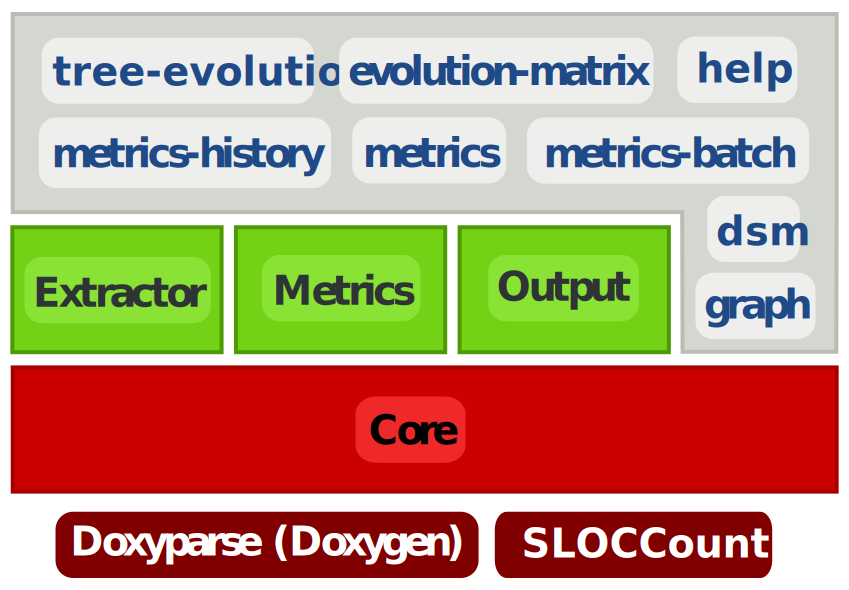
\includegraphics[scale=0.3]{imagens/analizo-architecture.png}
\caption{Arquitetura do Analizo, usando Layered Style \cite{Clements2002}}
\label{arquitetura-analizo}
\end{figure}

O {\it Core} contém as estruturas de dados usadas para armazenar informações a
respeito do código-fonte sendo analisado, como a lista de módulos\footnote{o
conceito ``módulo'' é usado como um termo abrangente para designar diferentes
tipos de estruturas usados em desenvolvimento de software, como classes e
arquivos fonte C}, elementos dentro de cada módulo (atributos, variáveis,
métodos, funções), informações de dependência (chamada, herança, etc). Esta
camada implementa a maior parte da lógica de negócio do Analizo, e não depende
de nenhuma outra camada.

A camada {\it Extractor} lida com as informaçoes de código-fonte obtidas pelas
diferentes estratégias implementadas no Analizo. Os extratores obtém
informações do código-fonte e armazenam em estruturas de dados da camada {\it
Core}. Adicionar um novo extrator requer apenas a criação de uma nova subclasse
que faça interface com uma ferramenta externa ou que ela própria realize análise
de código-fonte. Atualmente existem dois extratores, ambos fazem interface
com ferramentas externas de análise estática de código-fonte:

\begin{itemize}

  \item {\it Analizo::Extractor::Doxyparse} é uma interface para o Doxyparse,
  um parser de código-fonte para C, C++ e Java desenvolvida por nosso grupo de
  pesquisa\cite{Costa2009}. Doxyparse é baseado no
  Doxygen\footnote{doxygen.org}, um sistema de documentação multi-linguagem.

  \item {\it Analizo::Extractor::Sloccount} é uma interface para o
  Sloccount\footnote{dwheeler.com/sloccount} desenvolvido por David A. Wheeler,
  uma ferramenta que calcula o número efetivo de linhas de código.

\end{itemize}

As outras camadas intermediárias são {\it Metrics} e {\it Output}. A camada
{\it Metrics} processa as estruturas de dados do {\it Core} para calcular
métricas, até o momento Analizo suporta um conjunto razoável de métricas
(listadas na Seção \ref{metricas}), uma representação desta camada pode ser
vista no diagrama da Figura \ref{arquitetura-metrics-analizo}. A camada {\it
Output} é responsável por lidar com diferentes formatos de arquivos.
Atualmente, apenas o formato DOT é implementado no Analizo para representar
grafo de dependencia, adicionar novos formatos é simplesmente adicionar novas
classes nesta camada.

\begin{figure}[H]
\center
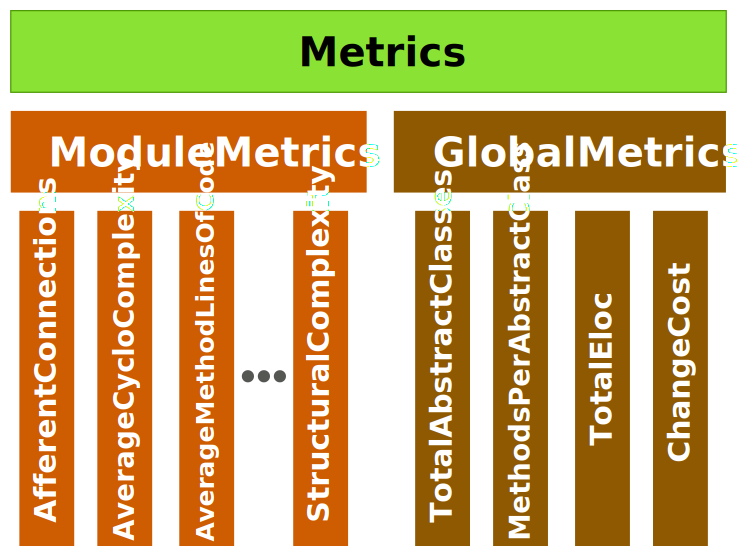
\includegraphics[scale=0.4]{imagens/analizo-metrics-architecture.png}
\caption{Arquitetura do módulo metrics em detalhe, usando Layered Style \cite{Clements2002}}
\label{arquitetura-metrics-analizo}
\end{figure}

A camada {\it Tools} fornece um conjunto de ferramentas de linha de comando que
constituem a interface do analizo, tanto para usuários finais quanto para
aplicações de mais alto nível. Estas ferramentas usam serviços providos pelas
outras camadas: eles instanciam as estruturas de dados do {\it Core},
inicializam um ou mais extratores, opcionalmente executam o processador de
métricas, instanciam um módulo de formato de saída, e gerencia todos eles para
prover o resultado desejado. A maioria das funcionalidades descritas na Seção
\ref{funcionalidades} são implementadas na camada {\it Tools} do Analizo.

Estas ferramentas são pensadas na filosofia UNIX: fazem uma tarefa
especializada e geram uma saída que pode ser utilizada como entrada para outras
ferramentas, seja para o próprio Analizo ou para ferramentas externas. Algumas das
ferramentas implementadas no Analizo são feitas consumindo saída gerada por
outra ferramenta ao invés de manipular explicitamente os internos do Analizo,
algumas outras são desenhadas para prover saída em formato específico para
aplicacoes externas, como por exemplo programas para desenho de grafos ou
visualização de dados.

\subsubsection{Funcionalidades}\label{funcionalidades}

{\bf Análise de código-fonte multi-linguagem}

Atualmente Analizo suporta análise de código-fonte escrito em C, C++ e Java.
Entretanto, pode ser facilmente estendido para suportar outras linguagens pois
pode potencialmente suportar as inúmeras outras linguagens suportadas pelo Doxygen.

{\bf Métricas}\label{metricas}

O Analizo suporta tanto métricas em nível de projeto, que é calculada para todo o projeto,
quanto métricas em nível de módulos, que é calculado individualmente para cada módulo.
No nível de projeto, Analizo também provê estatística descritiva básica para cada métrica em
nível de módulo: soma, média, mediana, moda, desvio padrão, variância, skewness e kurtosis da
distribuição, valores mínimo e maximo. As seguintes métricas são suportadas até o momento:

\begin{itemize}

  \item Métricas em nível de projeto: Change Cost, Total Abstract Classes,
  Total Coupling Factor, Total Effective Lines of Code, Total Lines of Code,
  Methods per Abstract Class, Total Number of Modules, Total number of modules
  with at least one defined attributes, Total number of modules with at least
  one defined method, Total Number of Methods.

  \item Métricas em nível de módulo: Afferent Connections per Class, Average
  Cyclomatic Complexity per Method, Average Method Lines of Code, Argument with
  'nonnull' attribute passed null, Average Number of Parameters per Method,
  Allocator sizeof operand mismatch, Assigned value is garbage or undefined,
  Bad deallocator, Bad free, Coupling Between Objects, Dead assignment,
  Divisions by zero, Double free, Depth of Inheritance Tree, Dereference of
  null pointer, Dereference of undefined pointer value, Potential buffer
  overflow in call to 'gets', Lack of Cohesion of Methods, Lines of Code,
  Memory leak, Max Method LOC, Number of Attributes, Number of Children, Number
  of Methods, Number of Public Attributes, Number of Public Methods,
  Out-of-bound array access, Offset free, Potential insecure temporary file in
  call 'mktemp', Response for a Class, Result of operation is garbage or
  undefined, Return of stack variable address, Stack address stored into global
  variable, Structural Complexity, Undefined allocation of 0 bytes,
  Use-after-free, Uninitialized argument value.

\end{itemize}

É possível especificar que certos diretórios dentro do projeto não devem ser
analisados, de forma que o Analizo ignore tais arquivos durante a análise e o
cálculo de métricas.

{\bf Processamento em lote}\label{lote}

A maioria dos estudos quantitativos em Engenharia de Software envolve aquisição
de métricas de código-fonte de um grande número de projetos, processar cada
projeto individualmente é pouco prático, passível de erros e difícil de
repetir. Analizo pode processar multiplos projetos em lote e produzir arquivo
de dados CSV com métricas de cada projeto, bem como um resumo com as métricas
em nível de projeto de todos os projetos. Estes arquivos de dados podem ser
facilmente importados em ferramentas de estatística ou planilhas para análise
futura. Esta capacidade de processar em lote pode também ser utilizada para
analisar várias versões de um mesmo projeto, especialmente útil em estudos
sobre evolução de software.

Este processamento em lote pode se beneficiar de processamento paralelo dando
mais agilidade e na análise e reduzindo o tempo total de processamento.  A
saída pode ser também escrita diretamente em um banco de dados relacional ao
invés de gerar arquivos CSV. Outro recurso voltado à performance é um sistema
de cache para as informações previamente calculadas, evitando repetição de
processamento.

{\bf Histórico de métricas}

Algumas vezes pesquisadores precisam processar o histórico de projetos de
software de uma forma mais escalável. Analizo pode processar repositórios de
controle de versão e prover arquivo de dados CSV com valores de métricas para
cada revisão onde o código-fonte foi alterado no projeto, ou pode também gravar
os valores diretamente num banco de dados ao invés de usar arquivos CSV. Repositórios Git e
Subversion são suportados diretamente, repositórios CVS devem ser convertidos
para Git de forma manual.

{\bf Grafo de dependência}

Analizo pode gerar saída com informações sobre dependência entre as entidades
do projeto em um formato adequado para processamento por ferramentas de
renderização de grafos do Graphviz\footnote{graphviz.org}. A Figura
\ref{sample-graph} apresenta um exemplo de grafo desenhado pela ferramenta {\it
dot} do Graphviz a partir da saída gerada pelo Analizo {\it graph}.

\begin{figure}[h]
\center
\includegraphics[scale=0.4]{imagens/sample-graph.png}
\caption{Exemplo de grafo de dependência}
\label{sample-graph}
\end{figure}

{\bf Matriz de evolução}

Outra funcionalidade útil do Analizo é a visualização de matrizes de evolução
\cite{Lanza2001}. Ao processar cada release de um projeto (ver Seção
\ref{lote}), o usuário pode solicitar a criação de uma matrix de evolução a
partir de arquivos de dados individuais. A Figura \ref{sample-evolution-matrix}
apresenta um exemplo de uma matrix produzida pelo Analizo.

\begin{figure}[h]
\center
\includegraphics[scale=0.2]{imagens/sample-evolution-matrix.png}
\caption{Exemplo de matrix de evolução}
\label{sample-evolution-matrix}
\end{figure}

{\bf Matriz de estrutura de projeto}

Uma funcionalidade recente do Analizo é a representação visual do
relacionamento entre os módulos do projeto em forma de uma Matriz de estrutura
de projeto ({\it Design Structure Matrix}) \cite{Maccormack2006}, uma DSM é a
representação de um grafo de dependência em forma de uma matriz quadrada. Um
exemplo gerado pelo Analizo pode ser visto na Figura \ref{sample-dsm}.

\begin{figure}[h]
\center
\includegraphics[scale=0.3]{imagens/sample-dsm.png}
\caption{Exemplo de matrix de estrutura de projeto}
\label{sample-dsm}
\end{figure}

\subsubsection{Uso em trabalhos de pesquisa}
\label{trabalhos-analizo}

Analizo tem sido extensivamente usada por nosso grupo de pesquisa em diversos
estudos:

\begin{itemize}

  \item \cite{Amaral2009} usou o grafo de dependencia gerado pelo Analizo para
  gerar uma matriz de evolução em um estudo de caso com o projeto VLC.

  \item \cite{Costa2009} fez uma comparação entre diferentes estratégias para
  extração de informação de dependencias entre módulos do código-fonte,
  resultando no desenvolvimento do Doxyparse - o extrator baseado no Doxygen do
  Analizo.

  \item \cite{Terceiro2009} usou métricas em um estudo exploratório sobre a
  evolução da complexidade estrutural em projetos de software livre escritos em
  C.

  \item \cite{Morais2009} usou a ferramenta de métricas do Analizo como backend
  para o Kalibro, um software para avaliação e observação de métricas de código-fonte.
  
  \item \cite{Terceiro2010} usou o processamento de histórico de métricas para
  realizar um estudo exploratório sobre a evolução da complexidade estrutural em
  7 projetos de servidor web de diferentes tamanhos.

  \item \cite{Meirelles2010} usou o processamento em lote do Analizo para
  processas o código-fonte de mais de 6000 projetos de software livre do
  repositório Sourceforge.net.

  \item \cite{Meirelles2011} usou o Analizo em um estudo sobre impacto de
  métricas de código-fonte na atratividade de projetos de softwares livres.

  \item \cite{Terceiro2012Understanding} usou o Analizo para investigar fatores
  que influenciam na evolução da complexidade estrutural em projetos de software
  livres.

  \item \cite{Silva2012} usou o Analizo para minerar 16000 revisões de
  repositórios de projetos de software para investigar o potencial de uma nova
  métrica chamada Lack of Concern-based Cohesion.

  \item \cite{Ronaldo2015} utilizou o Analizo para extrair métricas de
  código-fonte de 14 versões do sistema Android e estudar a evoluçao da API e
  seus aplicativos.

\end{itemize}

A maioria destes trabalhos contribuíram com melhorias para o Analizo, fazendo
dele ainda mais apropriado para pesquisas envolvendo análise de código-fonte.

\subsubsection{Considerações finais}

Analizo é útil tanto para pesquisadores trabalhando com análise de código-fonte
quanto para profissionais que precisam analisar seus projetos em busca de
potenciais problemas ou melhorias. Neste trabalho de mestrado utilizamos o
Analizo para coletar métricas de código-fonte das ferramentas de análise
estática selecionadas.

Analizo é software livre, licenciado sob a GNU General Public License versão 3.
Seu código-fonte, bem como pacotes binários, manuais e tutoriais podem ser
obtidos em http://analizo.org. Todas as ferramentas são auto-documentadas e
podem ser consultadas como páginas de manual UNIX. Analizo é escrito em Perl.
Sua última versão 1.19.1 foi lançada (no escopo deste trabalho) em 01 de
Setembro de 2016 e será a versão utilizada neste estudo.

\section{Análise dos dados} \label{analise}

Os dados coletados pelo Analizo incluem métricas de código-fonte para cada módulo/classe de
cada ferramenta selecionada, tanto da indústria quanto da academia. As
métricas a serem analisadas e interpretadas são as métricas descritas na Seção
\ref{metricas-de-codigo}.

A linguagem R \cite{Ihaka1996}, uma linguagem de programação para cálculos
estatísticos e gráficos, será utilizada para manipulação de dados, criação de
tabelas e plotagem de gráficos. Todos os cálculos em linguagem R utilizados
neste trabalho estão disponíveis
em nosso repositório\footnote{http://github.com/joenio/dissertacao-ufba-2016} no arquivo {\em dissertacao.R}\footnote{http://github.com/joenio/dissertacao-ufba-2016/blob/master/dissertacao.R}.

Numa primeira análise dos valores coletados pelo Analizo notamos uma anomalia
nos valores da métrica CBO, o que nos levou a investigar de perto os motivos,
esta anomalia se apresentava como valores extremamente altos para esta métrica,
bastante discrepante com as demais métricas calculadas.

Para entender se estes valores estavam corretor ou não, utilizamos uma outra
ferramenta para cálculo das métricas, em nossos estudos encontramos e
utilizamos uma versão de avaliação da ferramenta {\it SciTools
Understand}\footnote{http://scitools.com/trial-download-3} em sua versão
``4.0.853'' em Linux 64 bits. Os dados extraídos por esta ferramenta podem ser
encontrados em nosso
repositório\footnote{http://github.com/joenio/dissertacao-ufba-2016/tree/master/dataset/Understand
SciTools}. Eles demonstraram que os valores calculados pelo Analizo estavam
bastante alto em comparação com as demais métricas.

Assim, descobrimos que o Analizo tinha de fato um erro no cálculo da métrica
CBO, erro que foi corrigido durante este estudo e disponibilizado na versão
mais recente do Analizo, versão que está sendo utilizada aqui.

Com isto podemos analisar os dados das métricas para cada uma das ferramentas analisadas,
calculamos os percentis de cada métrica para cada ferramenta a partir dos
valores das métricas dos seus módulos, um percentil é a centésima parte dos
dados ordenados de forma crescente, iremos calcular os percentis 1, 5, 10, 25,
50, 75, 90, 95 e 99, e dentre eles iremos discutir os resultados em função dos
percentis 75, 90 e 95, assim como feito por \citeonline{Meirelles2013},
correspondendo a valores muito frequentes, frequentes e pouco frequentes,
respectivamente.

Estes intervalos serão
definidos a partir da interpretação manual dos percentis e serão analisados
usando modelos de regressão a fim de serem compreendidos e validados, uma
comparação com intervalos encontrados nos trabalhos relacionados (seção
\ref{trabalhos-relacionados}) também será realizada com objetivo de reforçar
estes valores.

Os valores encontrados serão avaliados sempre tendo em vista os intervalos
sugeridos na Tabela \ref{valores-frequentes}, esta tabela traz os valores encontrados
no estudo que estamos replicando em parte\cite{Meirelles2013}.

\begin{table}[H]
  \caption{Valores frequentes\cite{Meirelles2013}}
  \centering
  \begin{tabular}{| c | l | l | l | l | l |}
    \hline
    Métrica           & Linguagem & Muito frequente & Frequente & Pouco frequente & Não frequente \\
    \hline
\multirow{3}{*}{ACC}   & C         & 0 -- 2,0   & 2,1 -- 7,0   & 7,1 -- 13,0  & $>$ 13,0  \\
                       & C++       & 0 -- 2,0   & 2,1 -- 7,0   & 7,1 -- 13,0  & $>$ 13,0  \\
                       & Java      & 0 -- 2,0   & 2,1 -- 7,0   & 7,1 -- 13,0  & $>$ 13,0  \\
    \hline
\multirow{3}{*}{ACCM}  & C         & 0 -- 3,6   & 3,1 -- 5,3   & 5,4 -- 7,0   & $>$ 7,0   \\
                       & C++       & 0 -- 2,0   & 2,1 -- 4,0   & 4,1 -- 6,0   & $>$ 6,0   \\
                       & Java      & 0 -- 2,8   & 2,9 -- 4,4   & 4,5 -- 6,0   & $>$ 6,0   \\
    \hline
\multirow{3}{*}{AMLOC} & C         & 0 -- 15,6  & 15,7 -- 25,5 & 25,6 -- 39,3 & $>$ 39,3  \\
                       & C++       & 0 -- 8,0   & 9,0 -- 19,5  & 19,6 -- 37,0 & $>$ 37,0  \\
                       & Java      & 0 -- 8,3   & 8,4 -- 18,0  & 19,0 -- 34,0 & $>$ 34,0  \\
    \hline
\multirow{3}{*}{ANPM}  & C         & 0 -- 3,0   & 3,1 -- 4,0   & 4,1 -- 5,0   & $>$ 5,0   \\
                       & C++       & 0 -- 2,0   & 2,1 -- 3,0   & 3,1 -- 5,0   & $>$ 5,0   \\
                       & Java      & 0 -- 1,5   & 1,6 -- 2,0   & 2,1 -- 4,0   & $>$ 4,0   \\
    \hline
\multirow{3}{*}{CBO}   & C         & 0 -- 5,0   & 6,0 -- 9,0   & 9,0 -- 12,0  & $>$ 12,0  \\
                       & C++       & 0 -- 3,0   & 4,0 -- 5,0   & 6,0 -- 7,0   & $>$ 7,0   \\
                       & Java      & 0 -- 3,0   & 4,0 -- 6,0   & 7,0 -- 9,0   & $>$ 9,0   \\
    \hline
\multirow{3}{*}{DIT}   & C         & -          & -            & -            & -         \\
                       & C++       & 0 -- 1,0   & 2,0 -- 3,0   & 4,0          & $>$ 4,0   \\
                       & Java      & 0 -- 2,0   & 3,0 -- 4,0   & 5,0 -- 6,0   & $>$ 6,0   \\
    \hline
\multirow{3}{*}{LCOM4} & C         & 0 -- 5,0   & 6,0 -- 12,0  & 12,0 -- 20,0 & $>$ 20,0  \\
                       & C++       & 0 -- 5,0   & 6,0 -- 10,0  & 10,0 -- 14,0 & $>$ 14,0  \\
                       & Java      & 0 -- 3,0   & 4,0 -- 7,0   & 8,0 -- 12,0  & $>$ 12,0  \\
    \hline
\multirow{3}{*}{LOC}   & C       & 0 -- 79,0 & 80,0 -- 324,0 & 325,0 -- 877,0 & $>$ 877,0 \\
                       & C++      & 0 -- 31,0  & 32,0 -- 84,0 & 85,0 -- 207,0 & $>$ 207,0 \\
                       & Java     & 0 -- 33,0  & 34,0 -- 87,0 & 88,0 -- 200,0 & $>$ 200,0 \\
    \hline
\multirow{3}{*}{NOA}   & C         & 0 -- 9,0   & 10,0 -- 29,0 & 30,0 -- 57,0 & $>$ 57,0  \\
                       & C++       & 0 -- 4,0   & 5,0 -- 8,0   & 9,0 -- 13,0  & $>$ 13,0  \\
                       & Java      & 0 -- 3,0   & 4,0 -- 8,0   & 9,0 -- 12,0  & -         \\
    \hline
\multirow{3}{*}{NOC}   & C         & -          & -            & -            & -         \\
                       & C++       & 0          & 1,0          & 2,0          & $>$ 2,0   \\
                       & Java      & 0          & 1,0 -- 2,0   & 3,0          & $>$ 3,0   \\
    \hline
\multirow{3}{*}{NOM}   & C         & 0 -- 13,0  & 14,0 -- 29,0 & 30,0 -- 48,0 & $>$ 48,0  \\
                       & C++       & 0 -- 10,0  & 11,0 -- 17,0 & 18,0 -- 26,0 & $>$ 26,0  \\
                       & Java      & -          & -            & -            & -         \\
    \hline
\multirow{3}{*}{NPA}   & C         & 0          & 2,0          & 3,0 -- 5,0   & $>$ 5,0   \\
                       & C++       & 0          & 1,0          & 2,0 -- 4,0   & $>$ 4,0   \\
                       & Java      & 0          & 1,0          & 2,0 -- 3,0   & $>$ 3,0   \\
    \hline
\multirow{3}{*}{NPM}   & C         & 0 -- 2,0   & 3,0 -- 5,0   & 6,0 -- 14,0  & $>$ 14,0  \\
                       & C++       & 0 -- 3,0   & 4,0 -- 7,0   & 8,0 -- 13,0  & $>$ 13,0  \\
                       & Java      & -          & -            & -            & -         \\
    \hline

\multirow{3}{*}{RFC}   & C      & 0 -- 54,0  & 55,0 -- 152,0 & 153,0 -- 271,0 & $>$ 272,0 \\
                       & C++     & 0 -- 29,0  & 30,0 -- 64,0  & 65,0 -- 102,0 & $>$ 102,0 \\
                       & Java      & 0 -- 9,0   & 10,0 -- 26,0 & 27,0 -- 59,0 & $>$ 59,0  \\
    \hline
\multirow{3}{*}{SC}    & C         & 0 -- 18,0  & 19,0 -- 77,0 & 78,0 -- 168,0 & $>$ 168,0 \\
                       & C++       & 0 -- 12,0  & 13,0 -- 28,0 & 29,0 -- 51,0  & $>$ 51,0  \\
                       & Java      & 0 -- 6,0   & 7,0 -- 21,0  & 22,0 -- 45,0  & $>$ 45,0  \\
    \hline
  \end{tabular}
  \label{valores-frequentes}
\end{table}

% %% begin.rcode grafico-comparativo, fig.show='hold', fig.cap="distribuição dos percentis para todas ferramentas"
% % par(mfrow=c(3,2), oma=c(0,0,0,0))
% %
% % table = data.frame(percentis_by_project("accm"), percentis_by_nist_project("accm"))
% % matplot(table, type="l", pch=1, xlab="percentis", ylab="valor", xaxt="n", cex.lab=0.6, cex.axis=0.6, cex.sub=0.6, cex.main=0.6)
% % axis(1, at=1:length(rownames(table)), labels=rownames(table), cex.axis=0.6)
% % title(main="accm")
% %
% % table = data.frame(percentis_by_project("nom"), percentis_by_nist_project("nom"))
% % matplot(table, type="l", pch=1, xlab="percentis", ylab="valor", xaxt="n", cex.lab=0.6, cex.axis=0.6, cex.sub=0.6, cex.main=0.6)
% % axis(1, at=1:length(rownames(table)), labels=rownames(table), cex.axis=0.6)
% % title(main="nom")
% %
% % table = data.frame(percentis_by_project("lcom4"), percentis_by_nist_project("lcom4"))
% % matplot(table, type="l", pch=1, xlab="percentis", ylab="valor", xaxt="n", cex.lab=0.6, cex.axis=0.6, cex.sub=0.6, cex.main=0.6)
% % axis(1, at=1:length(rownames(table)), labels=rownames(table), cex.axis=0.6)
% % title(main="lcom4")
% %
% % table = data.frame(percentis_by_project("cbo"), percentis_by_nist_project("cbo"))
% % matplot(table, type="l", pch=1, xlab="percentis", ylab="valor", xaxt="n", cex.lab=0.6, cex.axis=0.6, cex.sub=0.6, cex.main=0.6)
% % axis(1, at=1:length(rownames(table)), labels=rownames(table), cex.axis=0.6)
% % title(main="cbo")
% %
% % table = data.frame(percentis_by_project("acc"), percentis_by_nist_project("acc"))
% % matplot(table, type="l", pch=1, xlab="percentis", ylab="valor", xaxt="n", cex.lab=0.6, cex.axis=0.6, cex.sub=0.6, cex.main=0.6)
% % axis(1, at=1:length(rownames(table)), labels=rownames(table), cex.axis=0.6)
% % title(main="acc")
% %
% % table = data.frame(percentis_by_project("sc"), percentis_by_nist_project("sc"))
% % matplot(table, type="l", pch=1, xlab="percentis", ylab="valor", xaxt="n", cex.lab=0.6, cex.axis=0.6, cex.sub=0.6, cex.main=0.6)
% % axis(1, at=1:length(rownames(table)), labels=rownames(table), cex.axis=0.6)
% % title(main="sc")
% %% end.rcode


%------------------------------------------%

\xchapter{Conclusões}{} \label{conclusoes}

\subsection{Seleção e caracterização das ferramentas}

\section{Próximos passos}

Os próximos passos estão concentrados no estudo dos valores de distribuição
das métricas nos percentis 75, 90 e 95, comparar os valores e comportamentos
encontrados em nossos dados com os trabalhos de referência sobre valores de
métricas de código-fonte e sua discussão sobre a qualidade interna.

Após esta análise inicial iremos adicionar mais ferramentas a partir de uma
nova revisão estruturada, e então atualizar os valores e discussões de forma a
refletir a inclusão das novas ferramentas selecionadas neste ciclo de revisão.

A partir daí teremos definição dos valores de referência para ferramentas de
análise estática de código-fonte, com isto iremos calcular quanto cada
ferramenta está distante dos valores de referência, isto dará indícios sobre a
qualidade interna de cada ferramenta.


%------------------------------------------%

\backmatter
\bibliography{bibliografia}

\appendix

\xchapter{Edições e endereços das conferências revisadas}{}
\label{edicoes-conferencias}

\section{SCAM - Source Code Analysis and Manipulation Working Conference}

\begin{itemize}
  \item SCAM 2001 - {\small http://ieeexplore.ieee.org/xpl/mostRecentIssue.jsp?punumber=7667}
  \item SCAM 2002 - {\small http://ieeexplore.ieee.org/xpl/mostRecentIssue.jsp?punumber=6494367}
  \item SCAM 2003 - {\small http://ieeexplore.ieee.org/xpl/mostRecentIssue.jsp?punumber=8773}
  \item SCAM 2004 - {\small http://ieeexplore.ieee.org/xpl/mostRecentIssue.jsp?punumber=9523}
  \item SCAM 2005 - {\small http://ieeexplore.ieee.org/xpl/mostRecentIssue.jsp?punumber=10344}
  \item SCAM 2006 - {\small http://ieeexplore.ieee.org/xpl/mostRecentIssue.jsp?punumber=4026839}
  \item SCAM 2007 - {\small http://ieeexplore.ieee.org/xpl/mostRecentIssue.jsp?punumber=4362882}
  \item SCAM 2008 - {\small http://ieeexplore.ieee.org/xpl/mostRecentIssue.jsp?punumber=4637522}
  \item SCAM 2009 - {\small http://ieeexplore.ieee.org/xpl/mostRecentIssue.jsp?punumber=5279860}
  \item SCAM 2010 - {\small http://ieeexplore.ieee.org/xpl/mostRecentIssue.jsp?punumber=5600365}
  \item SCAM 2011 - {\small http://ieeexplore.ieee.org/xpl/mostRecentIssue.jsp?punumber=6063701}
  \item SCAM 2012 - {\small http://ieeexplore.ieee.org/xpl/mostRecentIssue.jsp?punumber=6389882}
  \item SCAM 2013 - {\small http://ieeexplore.ieee.org/xpl/mostRecentIssue.jsp?punumber=6636284}
  \item SCAM 2014 - {\small http://ieeexplore.ieee.org/xpl/mostRecentIssue.jsp?punumber=6970367}
  \item SCAM 2015 - {\small http://ieeexplore.ieee.org/xpl/mostRecentIssue.jsp?punumber=7321933}
\end{itemize}

\section{ASE - Automated Software Engineering}

Até o ano de 1996 a conferencia ASE se chamava KBSE - Knowledge-Based Software
Engineering Conference e a partir de 1997 passou a se chamar ASE - Automated
Software Conference.

\begin{itemize}
  \item ASE/KBSE 1991 - {\small http://ieeexplore.ieee.org/xpl/mostRecentIssue.jsp?punumber=5069}
  \item ASE/KBSE 1992 - {\small http://ieeexplore.ieee.org/xpl/mostRecentIssue.jsp?punumber=421}
  \item ASE/KBSE 1993 - {\small http://ieeexplore.ieee.org/xpl/mostRecentIssue.jsp?punumber=921}
  \item ASE/KBSE 1994 - {\small http://ieeexplore.ieee.org/xpl/mostRecentIssue.jsp?punumber=995}
  \item ASE/KBSE 1995 - {\small http://ieeexplore.ieee.org/xpl/mostRecentIssue.jsp?punumber=3518}
  \item ASE/KBSE 1996 - {\small http://ieeexplore.ieee.org/xpl/mostRecentIssue.jsp?punumber=4065}
  \item ASE 1997 - {\small http://ieeexplore.ieee.org/xpl/mostRecentIssue.jsp?punumber=5003}
  \item ASE 1998 - {\small http://ieeexplore.ieee.org/xpl/mostRecentIssue.jsp?punumber=5935}
  \item ASE 1999 - {\small http://ieeexplore.ieee.org/xpl/mostRecentIssue.jsp?punumber=6516}
  \item ASE 2000 - {\small http://ieeexplore.ieee.org/xpl/mostRecentIssue.jsp?punumber=7013}
  \item ASE 2001 - {\small http://ieeexplore.ieee.org/xpl/mostRecentIssue.jsp?punumber=7763}
  \item ASE 2002 - {\small http://ieeexplore.ieee.org/xpl/mostRecentIssue.jsp?punumber=8183}
  \item ASE 2003 - {\small http://ieeexplore.ieee.org/xpl/conhome.jsp?punumber=1000064}
  \item ASE 2004 - {\small http://ieeexplore.ieee.org/xpl/mostRecentIssue.jsp?punumber=9305}
  \item ASE 2005 - {\small http://dl.acm.org/citation.cfm?id=1101908}
  \item ASE 2006 - {\small http://ieeexplore.ieee.org/xpl/mostRecentIssue.jsp?punumber=4019543}
  \item ASE 2007 - {\small http://dl.acm.org/citation.cfm?id=1321631}
  \item ASE 2008 - {\small http://ieeexplore.ieee.org/xpl/mostRecentIssue.jsp?punumber=4639292}
  \item ASE 2009 - {\small http://ieeexplore.ieee.org/xpl/mostRecentIssue.jsp?punumber=5431684}
  \item ASE 2010 - {\small http://dl.acm.org/citation.cfm?id=1858996}
  \item ASE 2011 - {\small http://ieeexplore.ieee.org/xpl/mostRecentIssue.jsp?punumber=6093623}
  \item ASE 2012 - {\small http://ieeexplore.ieee.org/xpl/mostRecentIssue.jsp?punumber=6494367}
  \item ASE 2013 - {\small http://ieeexplore.ieee.org/xpl/mostRecentIssue.jsp?punumber=6684409}
  \item ASE 2014 - {\small http://dl.acm.org/citation.cfm?id=2642937}
  \item ASE 2015 - {\small http://ieeexplore.ieee.org/xpl/mostRecentIssue.jsp?punumber=7371449}
\end{itemize}


%------------------------------------------%

\end{document}

% vim: filetype=tex
